\documentclass[10pt,a4paper]{book}
\usepackage{amsmath}
\usepackage{amsfonts}
\usepackage{amssymb}
\usepackage[english]{babel}
\usepackage{float}
\usepackage[left=2cm,right=2cm,top=2cm,bottom=2cm]{geometry}
\usepackage{graphicx}
\usepackage{hyperref} % Used for external links
\usepackage[utf8]{inputenc}
\usepackage{listings} % Used for source code listing
\usepackage{mathtools}

\setcounter{tocdepth}{3}

% Source code listing's parameters
\lstset{
  frame=single,
  keepspaces=true,
%  title=\lstname
}

\title{Second SPICE Exercise\\{\small{Fundamentals Of Electronics - a.a. 2018-2019 -
University of Padua (Italy)}}}
\author{Pietro Prandini (mat. 1097752)}

\begin{document}
\maketitle

\vspace*{\fill}
% License
\begin{center}
\tiny{This work is licensed under the Creative Commons Attribution-ShareAlike 4.0 International License. To view a copy of this license, visit \href{http://creativecommons.org/licenses/by-sa/4.0/}{http://creativecommons.org/licenses/by-sa/4.0/} or send a letter to Creative Commons, PO Box 1866, Mountain View, CA 94042, USA.}
\end{center}

\tableofcontents

\chapter{NMOS common source amplifier with bypass capacitance}
\begin{figure}[h]
  \centering
  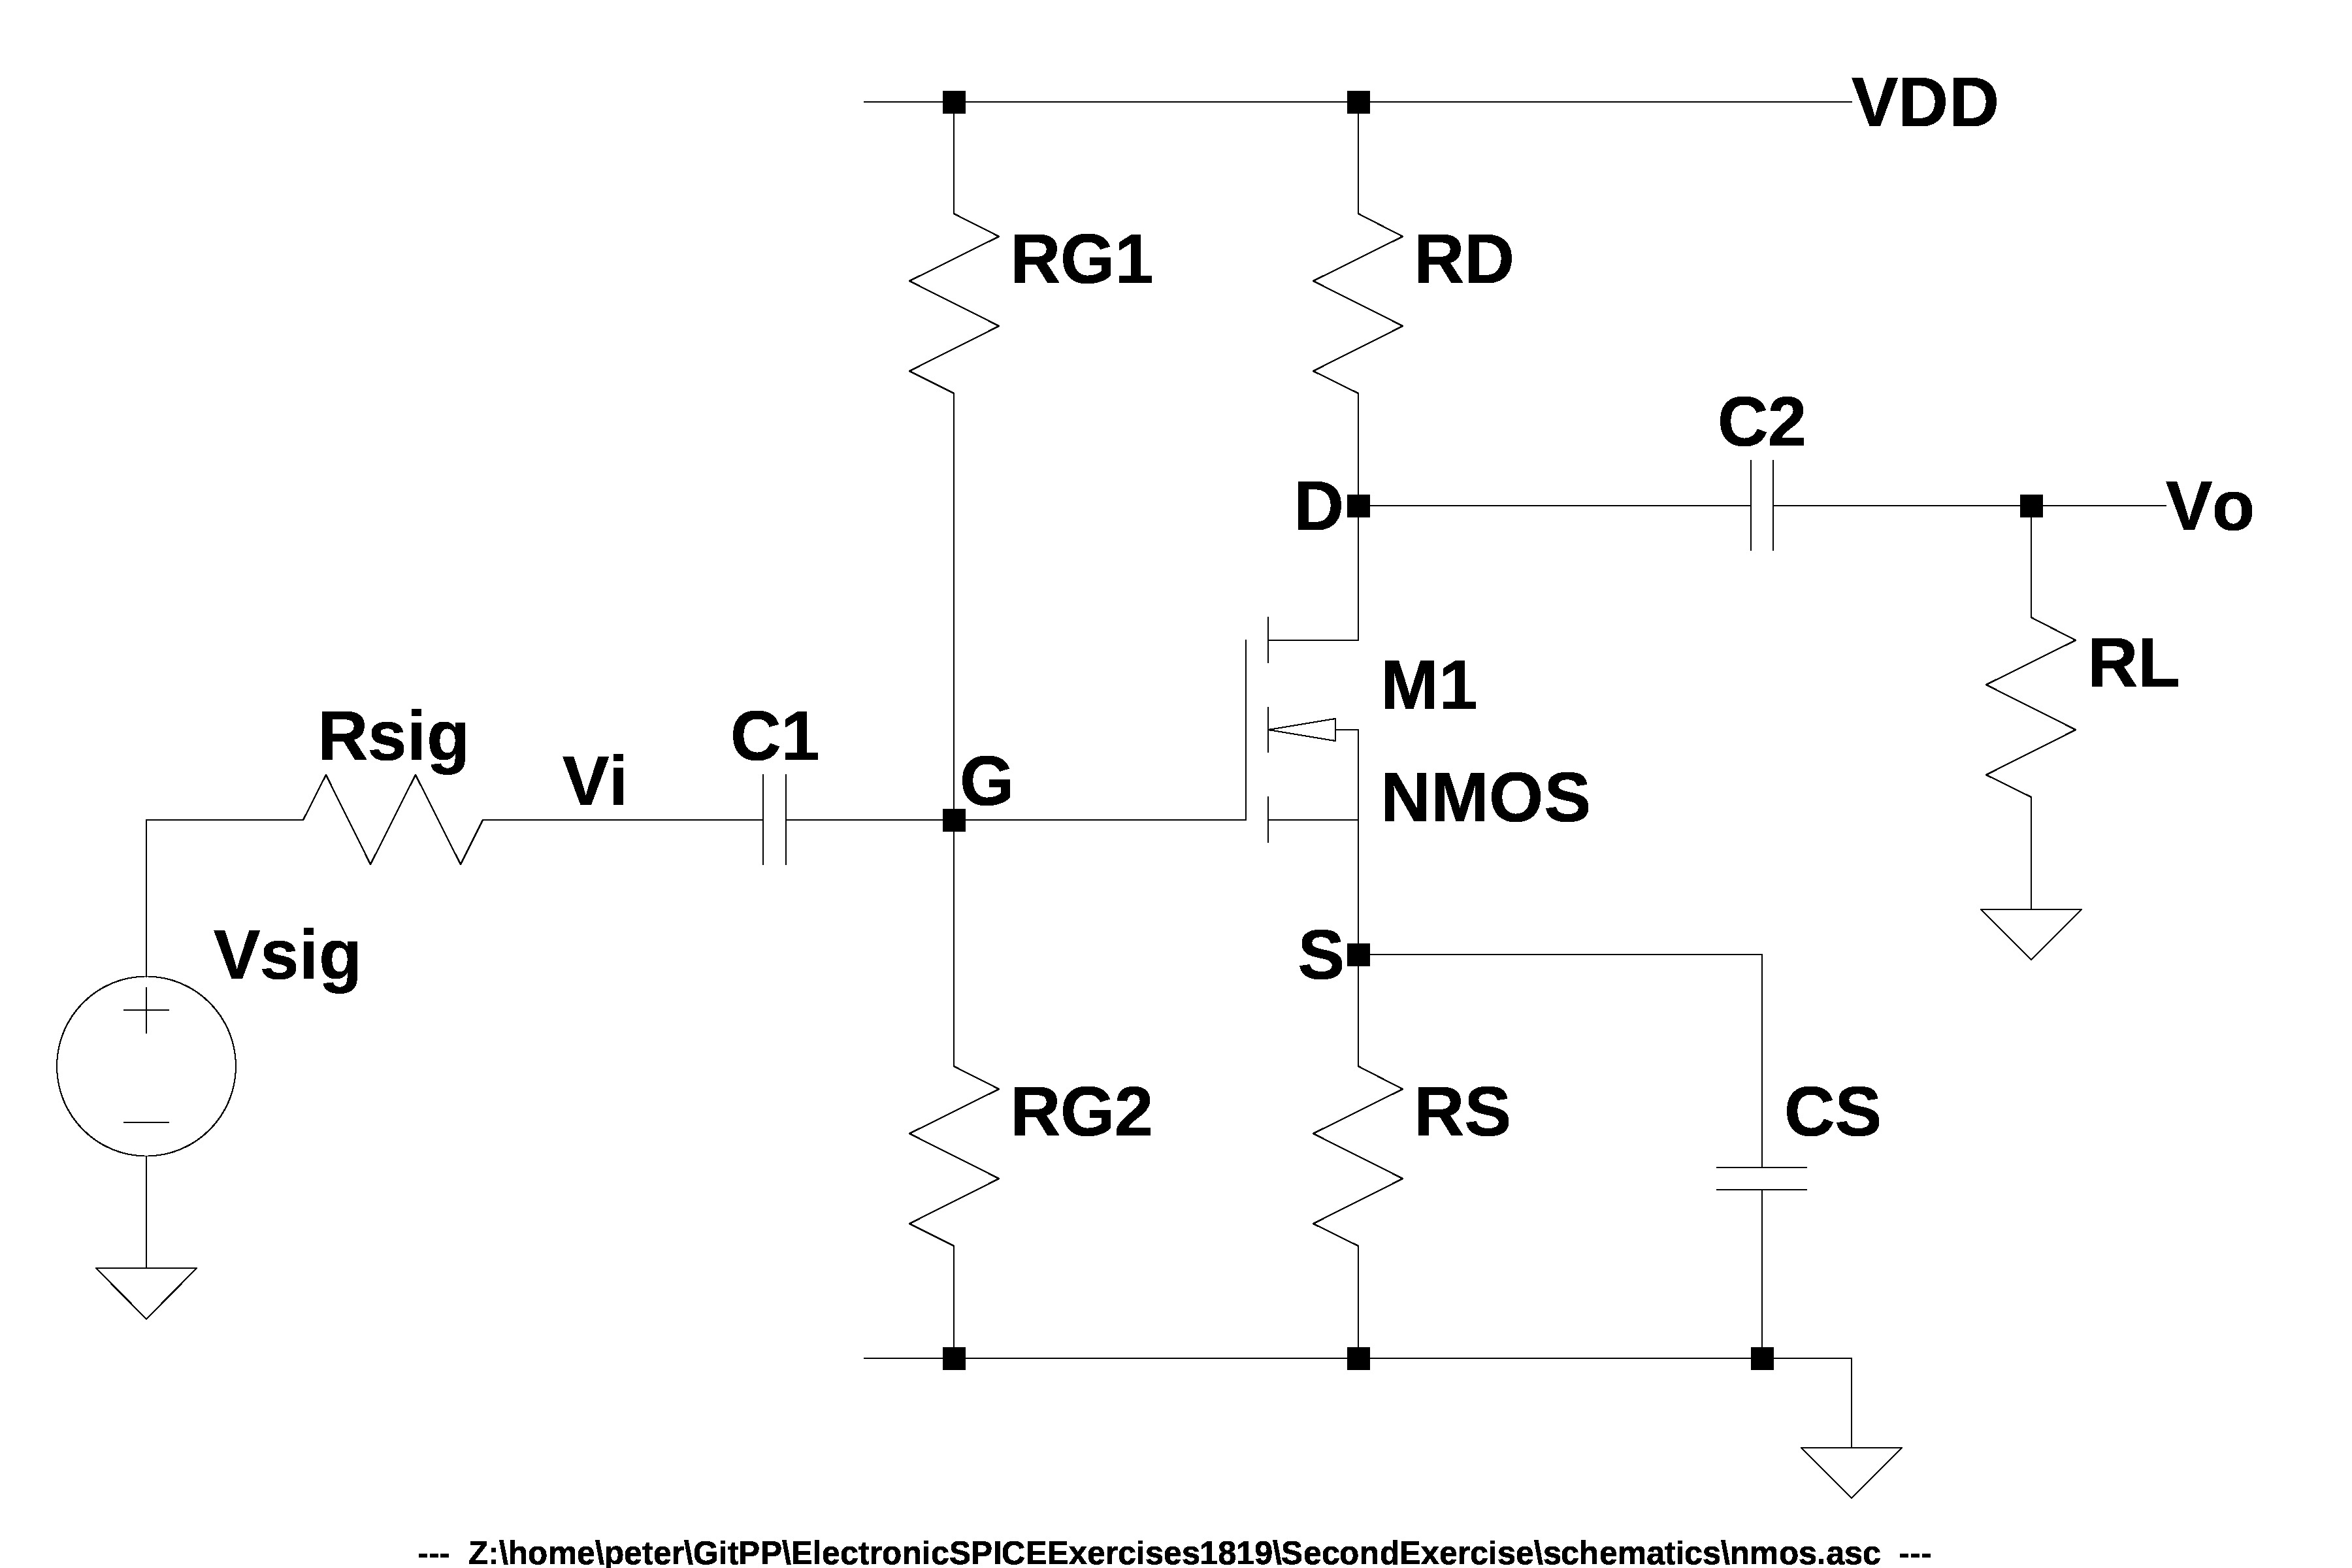
\includegraphics[width=12cm]{schematics/nmos.jpg}
  \caption{NMOS common source amplifier}
  \label{nmos}
\end{figure}

Designing the common source amplifier of the figure \ref{nmos} .\\
The MOSFET should have a $V_t = 1V$, a $K_n = 4mA/V$ and a $\lambda = 0$.\\
Other requested parameters are: $I_{DQ} = 0.5mA$, $V_S = 3.5V$, $V_D = 11V$, $V_{DD} = 15V$ and $R_{G2} = 1097752\Omega$.\par

\section{Analytic solutions}

\subsection{DC analysis}\label{nmos_DC_section}\label{DCsec}
On a Direct Current analysis the capacitances can be considered as open circuits, the inductances can be considered as short circuits, the signal and the load are removed and the alternate current inputs are not considered.\\
The figure \ref{nmos_DC} represents the circuit for the DC analysis.\par

\begin{figure}[h]
  \centering
  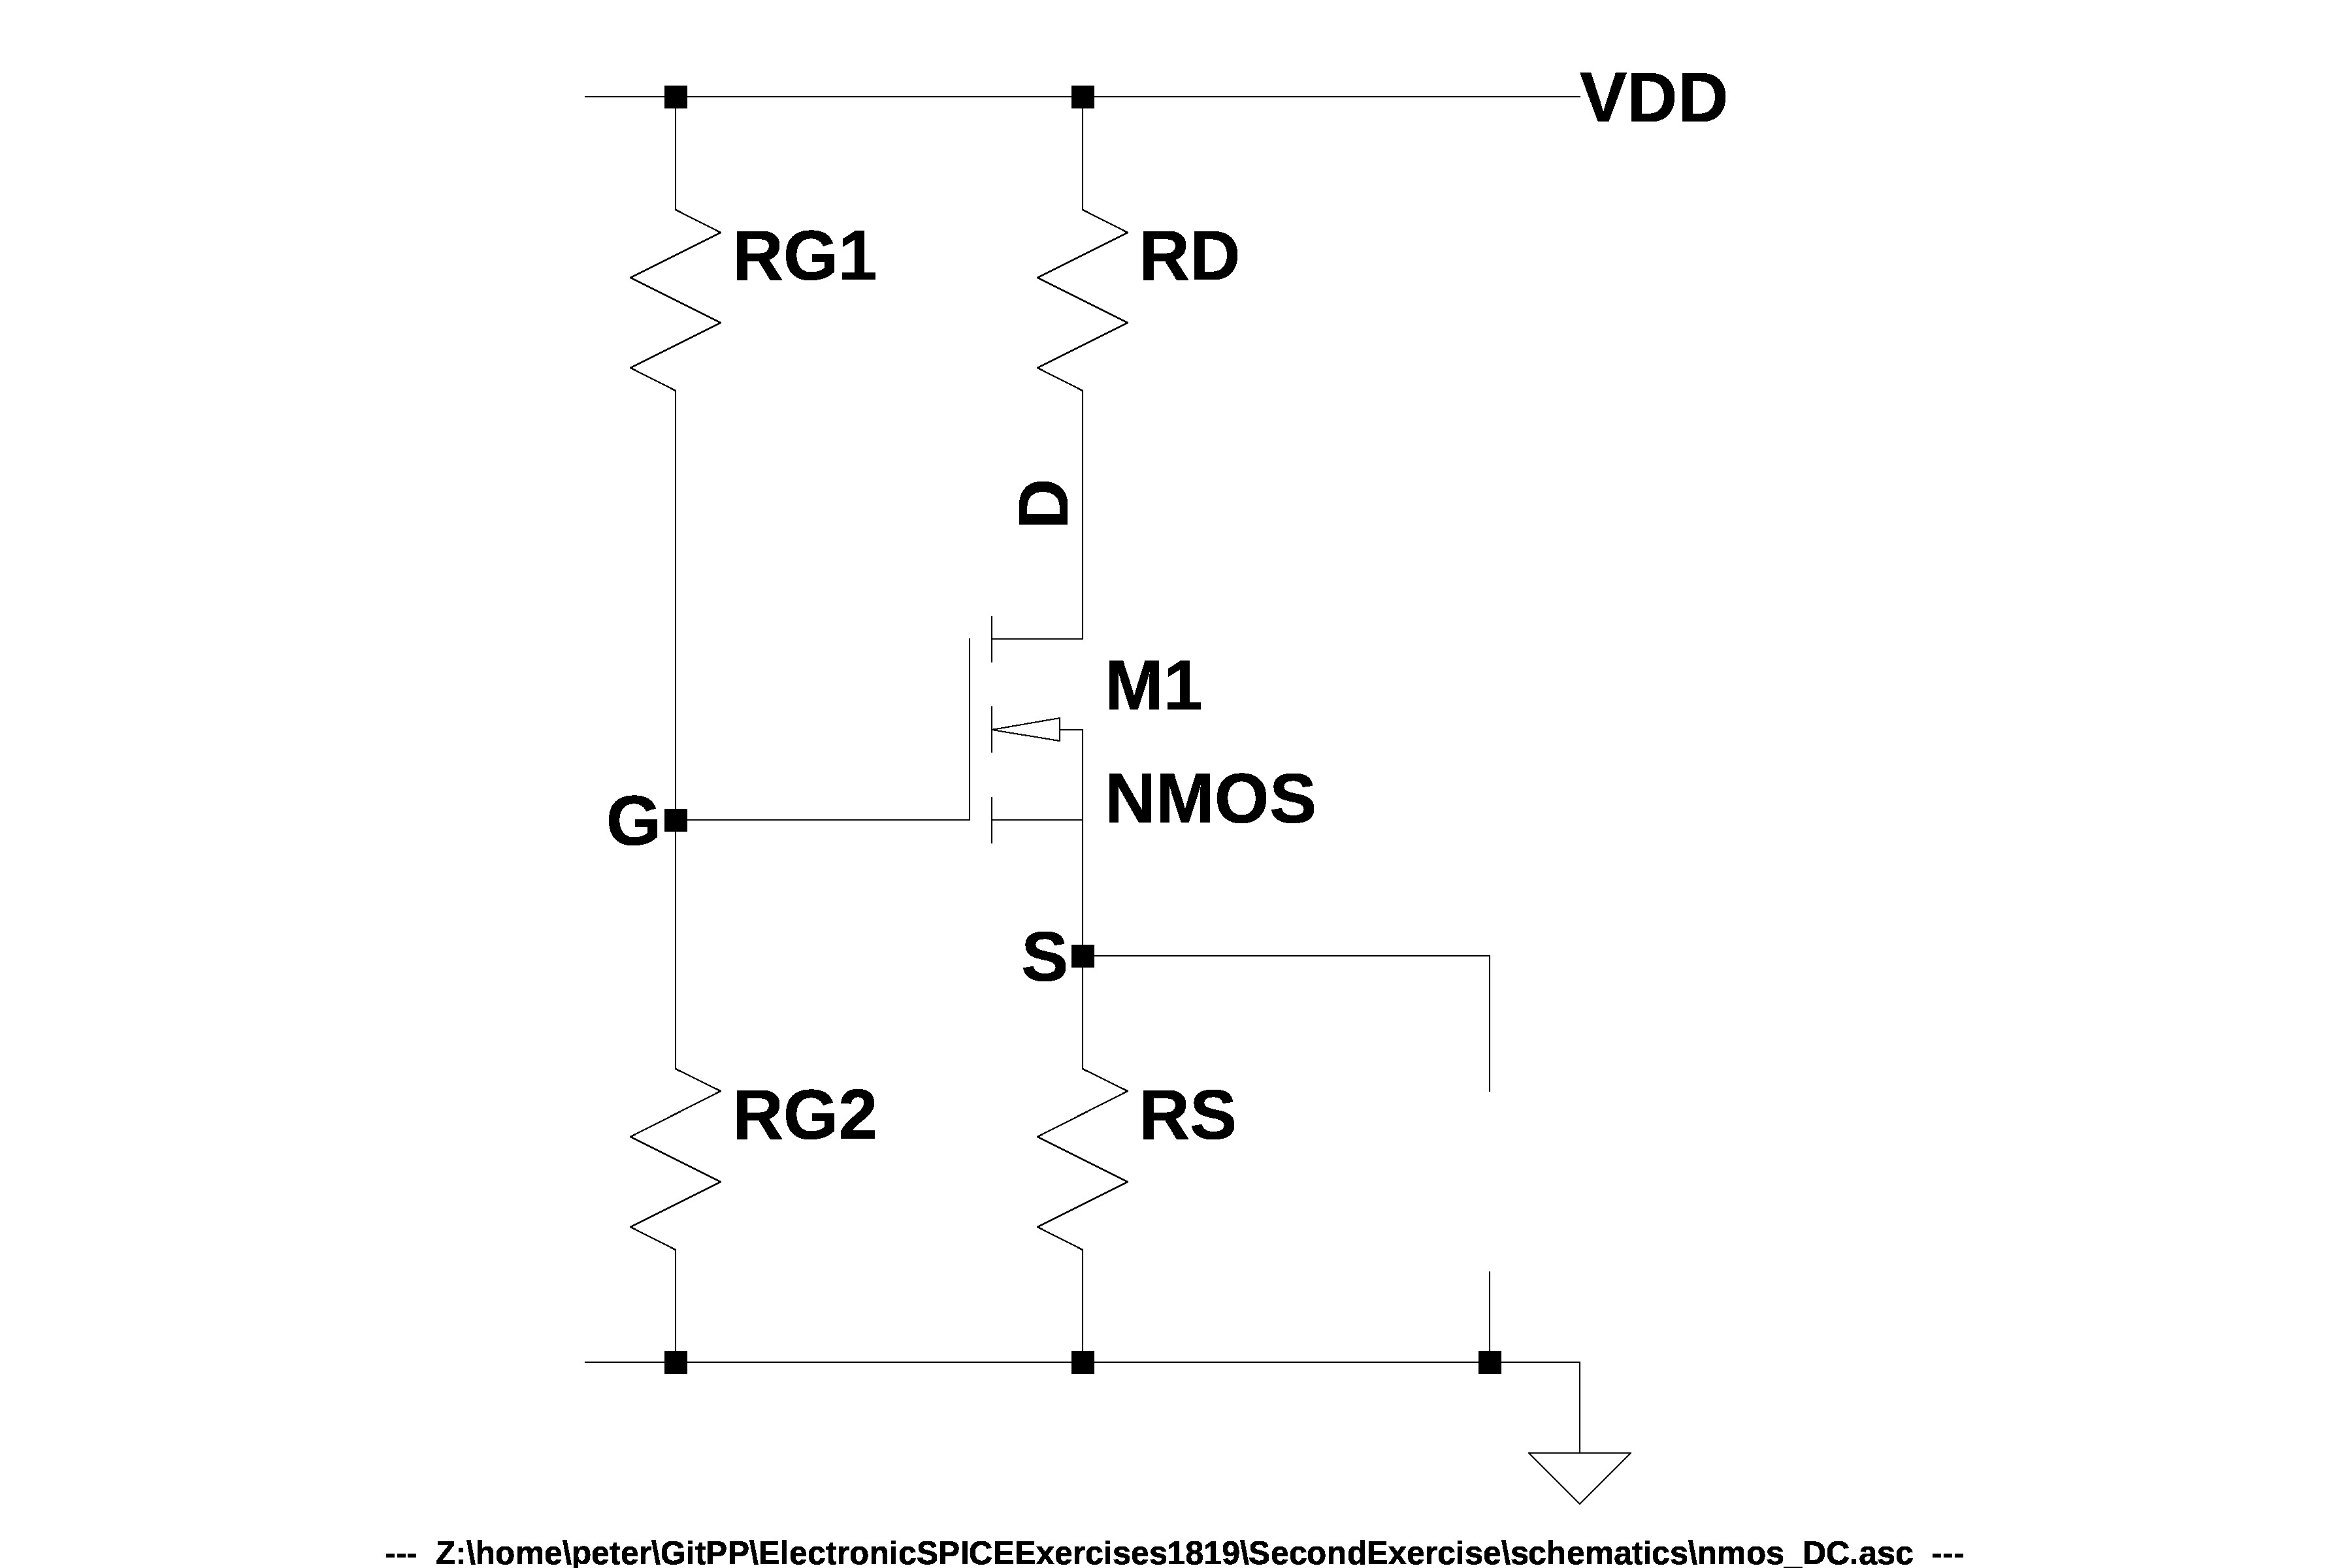
\includegraphics[width=12cm]{schematics/nmos_DC.jpg}
  \caption{NMOS common source amplifier - DC analysis}
  \label{nmos_DC}
\end{figure}

\subsubsection{$R_D$}
\begin{align}
V_{D} &= V_{DD} - R_D I_D\\
R_D &= \frac{V_{DD} - V_D}{I_D}\\
R_D &= \frac{15V - 11V}{0.5mA} = 8k\Omega
\end{align}

\subsubsection{$R_S$}
\begin{align}
V_S = R_S I_D \implies 
R_S = \frac{V_S}{I_D}\\
R_S = \frac{3.5V}{0.5mA} = 7k\Omega
\end{align}

\subsubsection{$V_{GS}$}
\begin{align}
I_D = \frac{1}{2}K_nV_{ov}^2 \implies
V_{ov} = \pm \sqrt{\frac{2 I_D}{K_n}}\\
V_{ov} = \pm \sqrt{\frac{2 \cdot 0.5mA}{4 mA/V^2}}\\
V_{ov} =
\left\{\begin{array}{l}
  + 0.5V \quad \text{Real value of } V_{ov} \text{.}\\
  - 0.5V \quad \text{No physical sense.}\\
\end{array}\right.
\end{align}
\begin{align}
V_{ov} = V_{GS} - V_{t} \implies
V_{GS} = V_{ov} + V_{t}\\
V_{GS} = 0.5V + 1V = 1.5V
\end{align}

\subsubsection{$R_{G1}$}
\begin{align}
V_{GS} = V_G - V_S \implies
V_G = V_{GS} + V_S\\
V_G = 1.5V + 3.5V = 5V
\end{align}

\begin{align}
I_G R_{G2} - V_{GS} - I_D R_S = 0 \implies
I_G = \frac{V_{GS}+I_D R_S}{R_{G2}}\\
I_G = \frac{1.5V + 0.5mA \cdot 7k\Omega}{1097.752k\Omega} = 4.5547628\mu A \simeq 4.55 \mu A
\end{align}

\begin{align}
R_{G1} &= \frac{V_{DD} - V_G}{I_G}\\
&= \frac{15V - 5V}{4.5547628 \mu A}\\
&=2.19550 M\Omega \simeq 2.20 M\Omega
\end{align}

\subsubsection{$g_m$}
\begin{align}
g_m = K_n V_{ov} = 4 mA/V^2 \cdot 0.5V = 2 mA/V
\end{align}

\subsubsection{$r_0$}
\begin{gather}
r_0 = \frac{1}{\lambda I_D} \xRightarrow{\lambda = 0} r_0 = \infty  \quad r_0 \text{ is considered as an open circuit.}
\end{gather}


\subsection{AC analysis}
On an Alternate Current analysis the capacitances can be considered as short circuits, the inductances can be considered as open circuits and the direct current inputs are not considered.\\
The figure \ref{nmos_AC} represents the circuit for the AC analysis.\\
Other requested parameters are: $R_{sig} = 200k\Omega$ and $R_L = 8k\Omega$.\par

\begin{figure}[h]
  \centering
  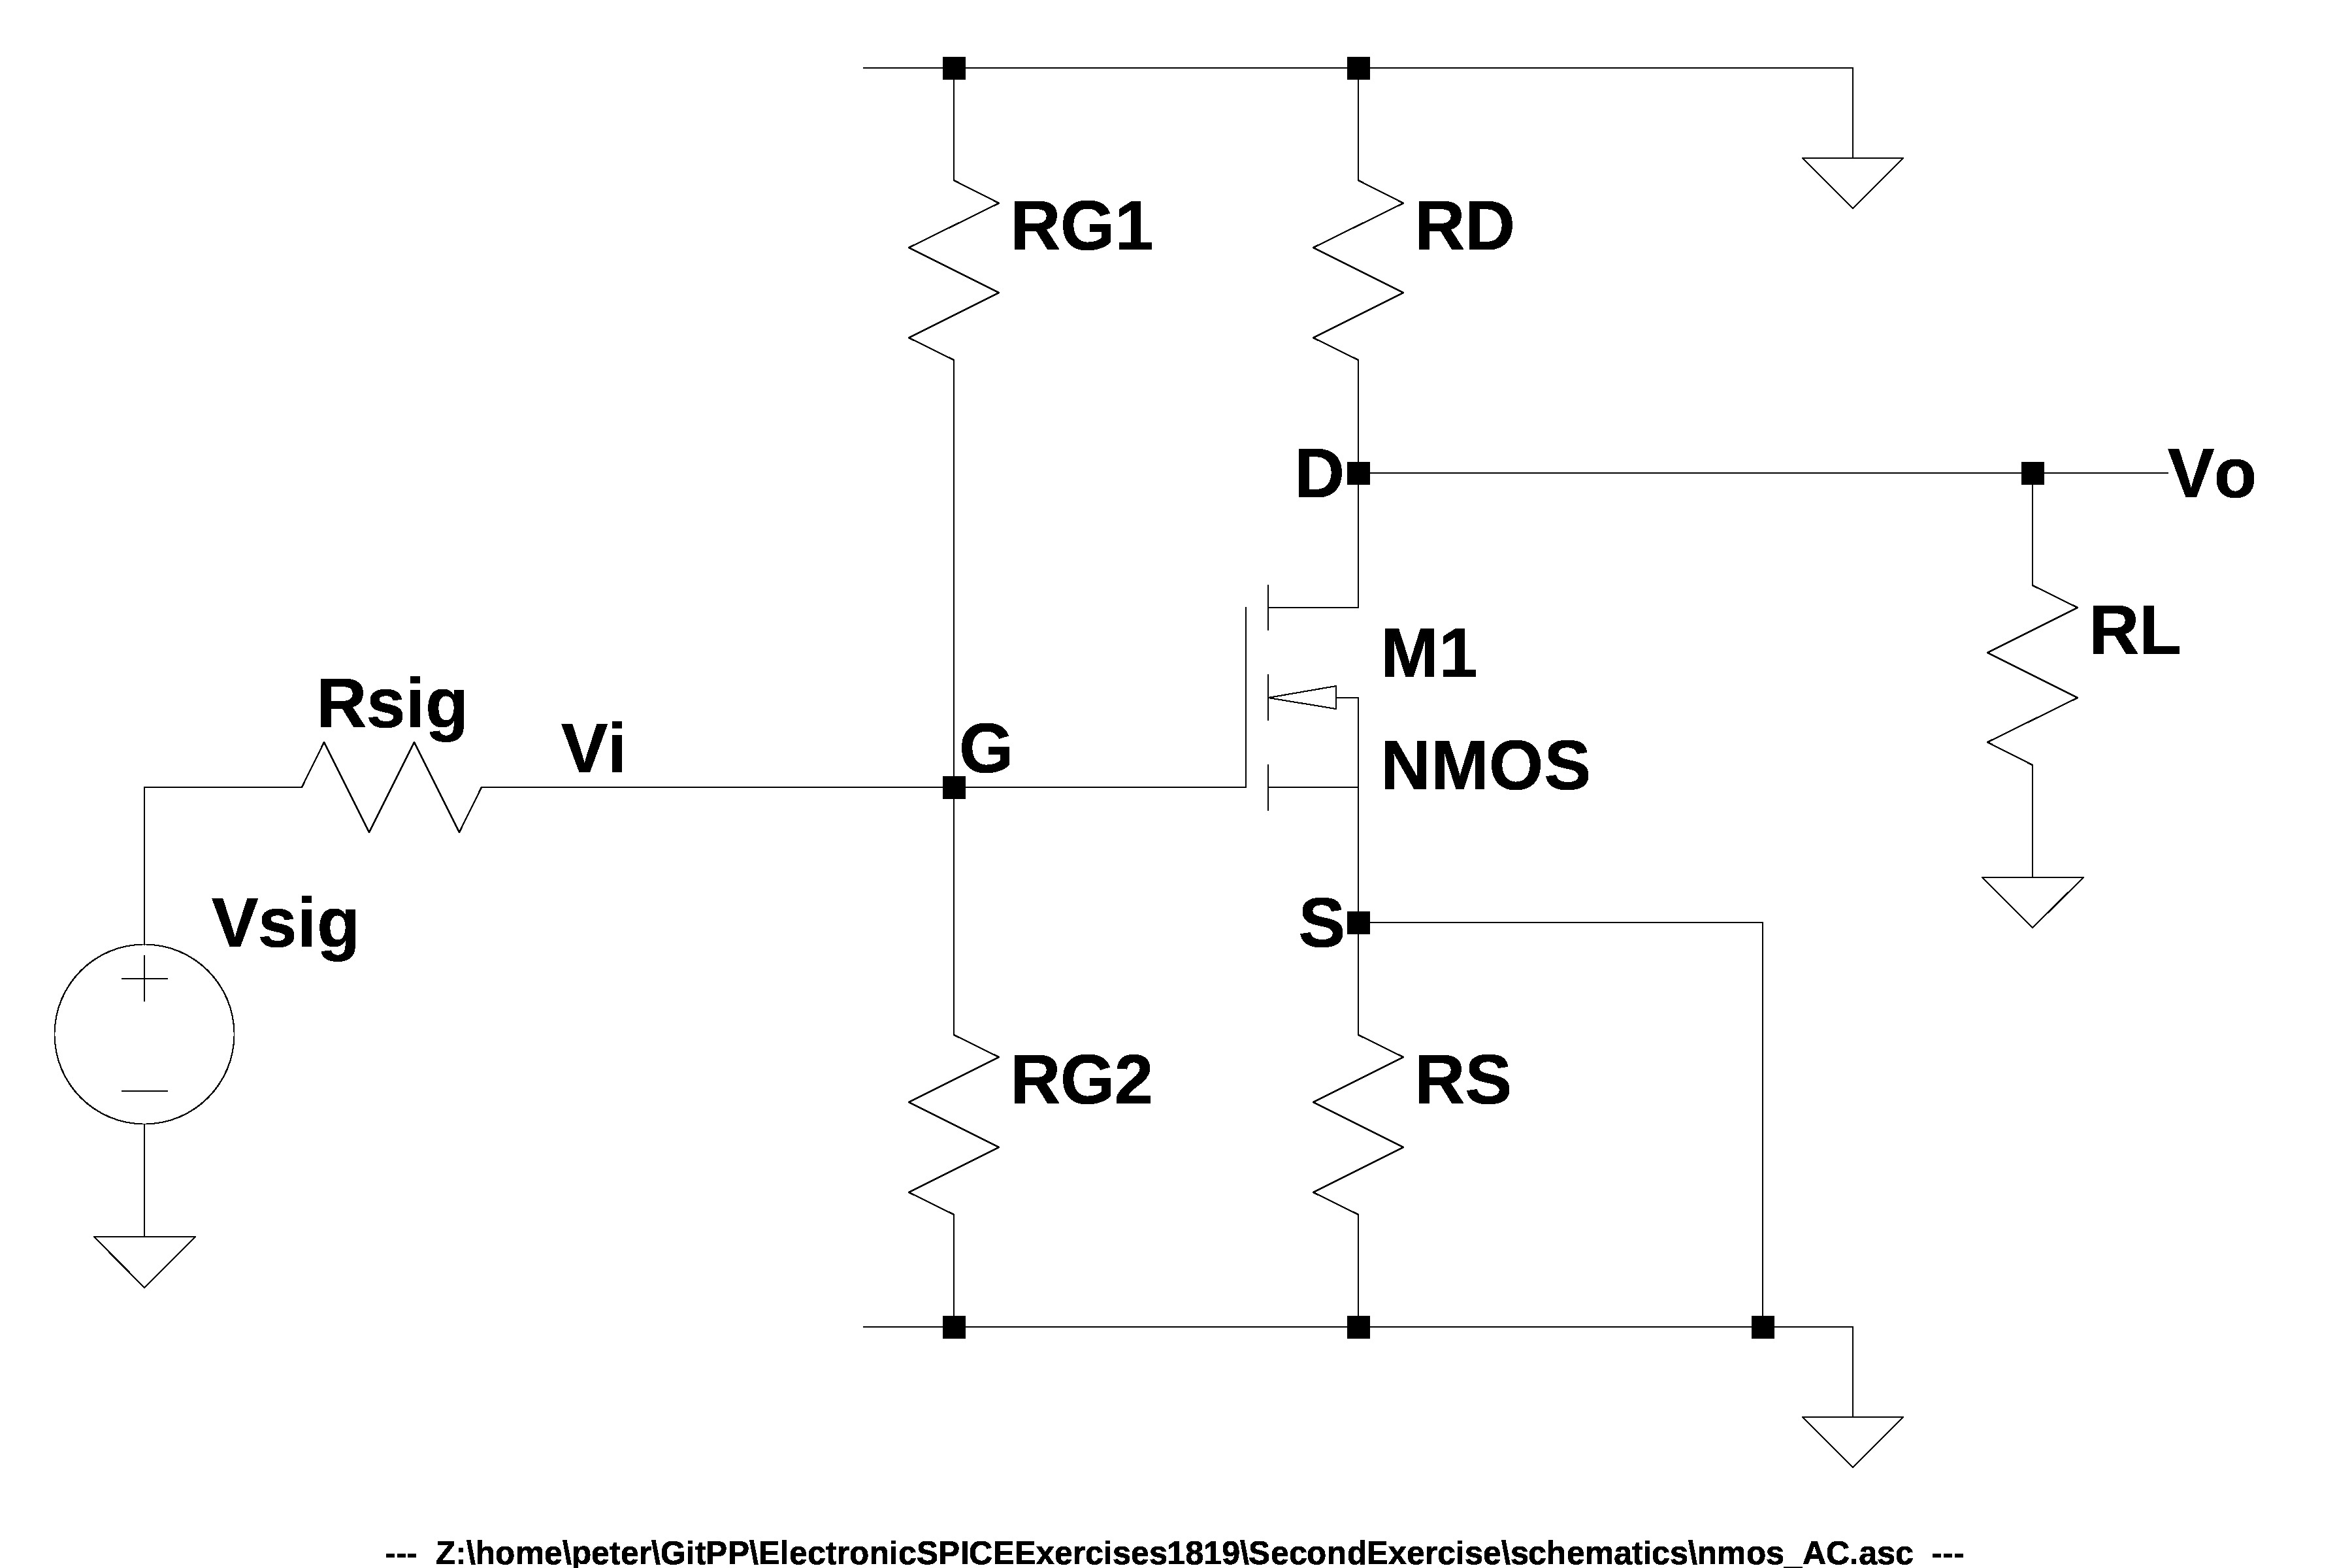
\includegraphics[width=12cm]{schematics/nmos_AC.jpg}
  \caption{NMOS common source amplifier - AC analysis}
  \label{nmos_AC}
\end{figure}

\subsubsection{Hybrid $\pi$ model}
For a small signal analysis it can be used an equivalent model to represent the behaviour of the transistor.\\
In this case it is used the hybrid $\pi$ model (figure \ref{nmos_pi}).\par

\begin{figure}[h]
  \centering
  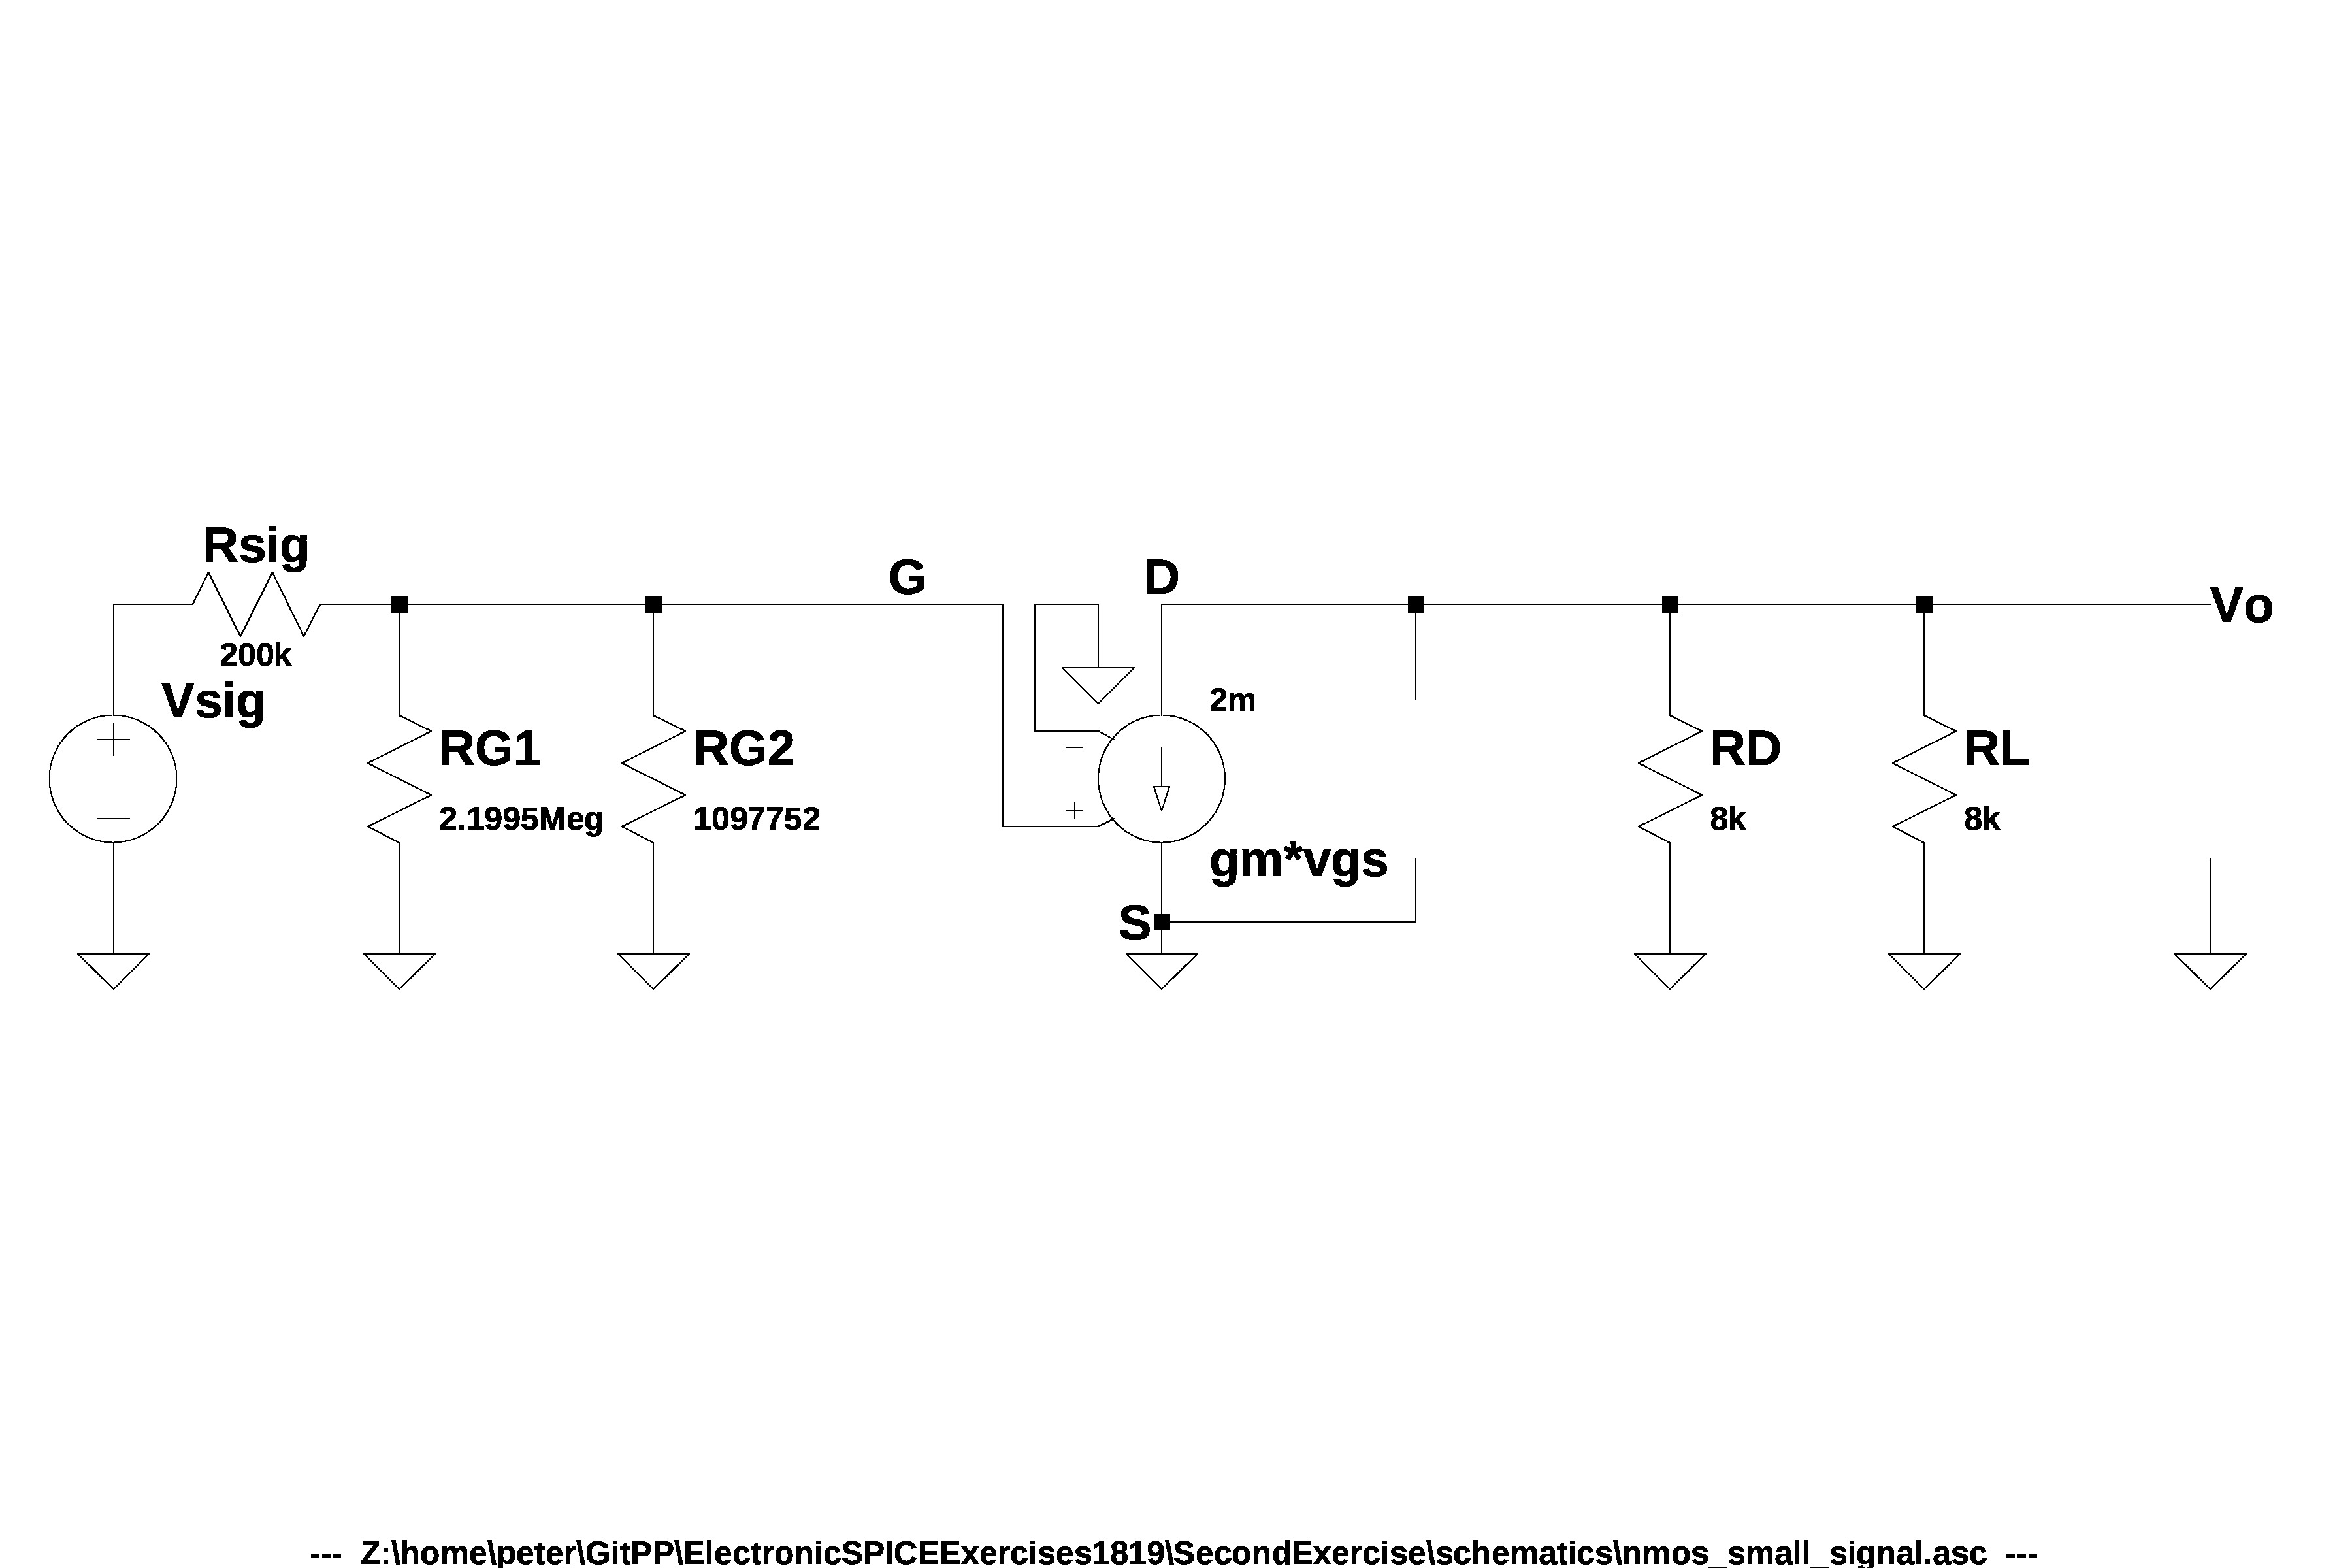
\includegraphics[width=12cm]{schematics/nmos_small_signal.jpg}
  \caption{NMOS common source amplifier - Hybrid $\pi$ model}
  \label{nmos_pi}
\end{figure}

\subsubsection{$R_{IN}$ from $G$}\label{RIN}

\begin{figure}[h]
  \centering
  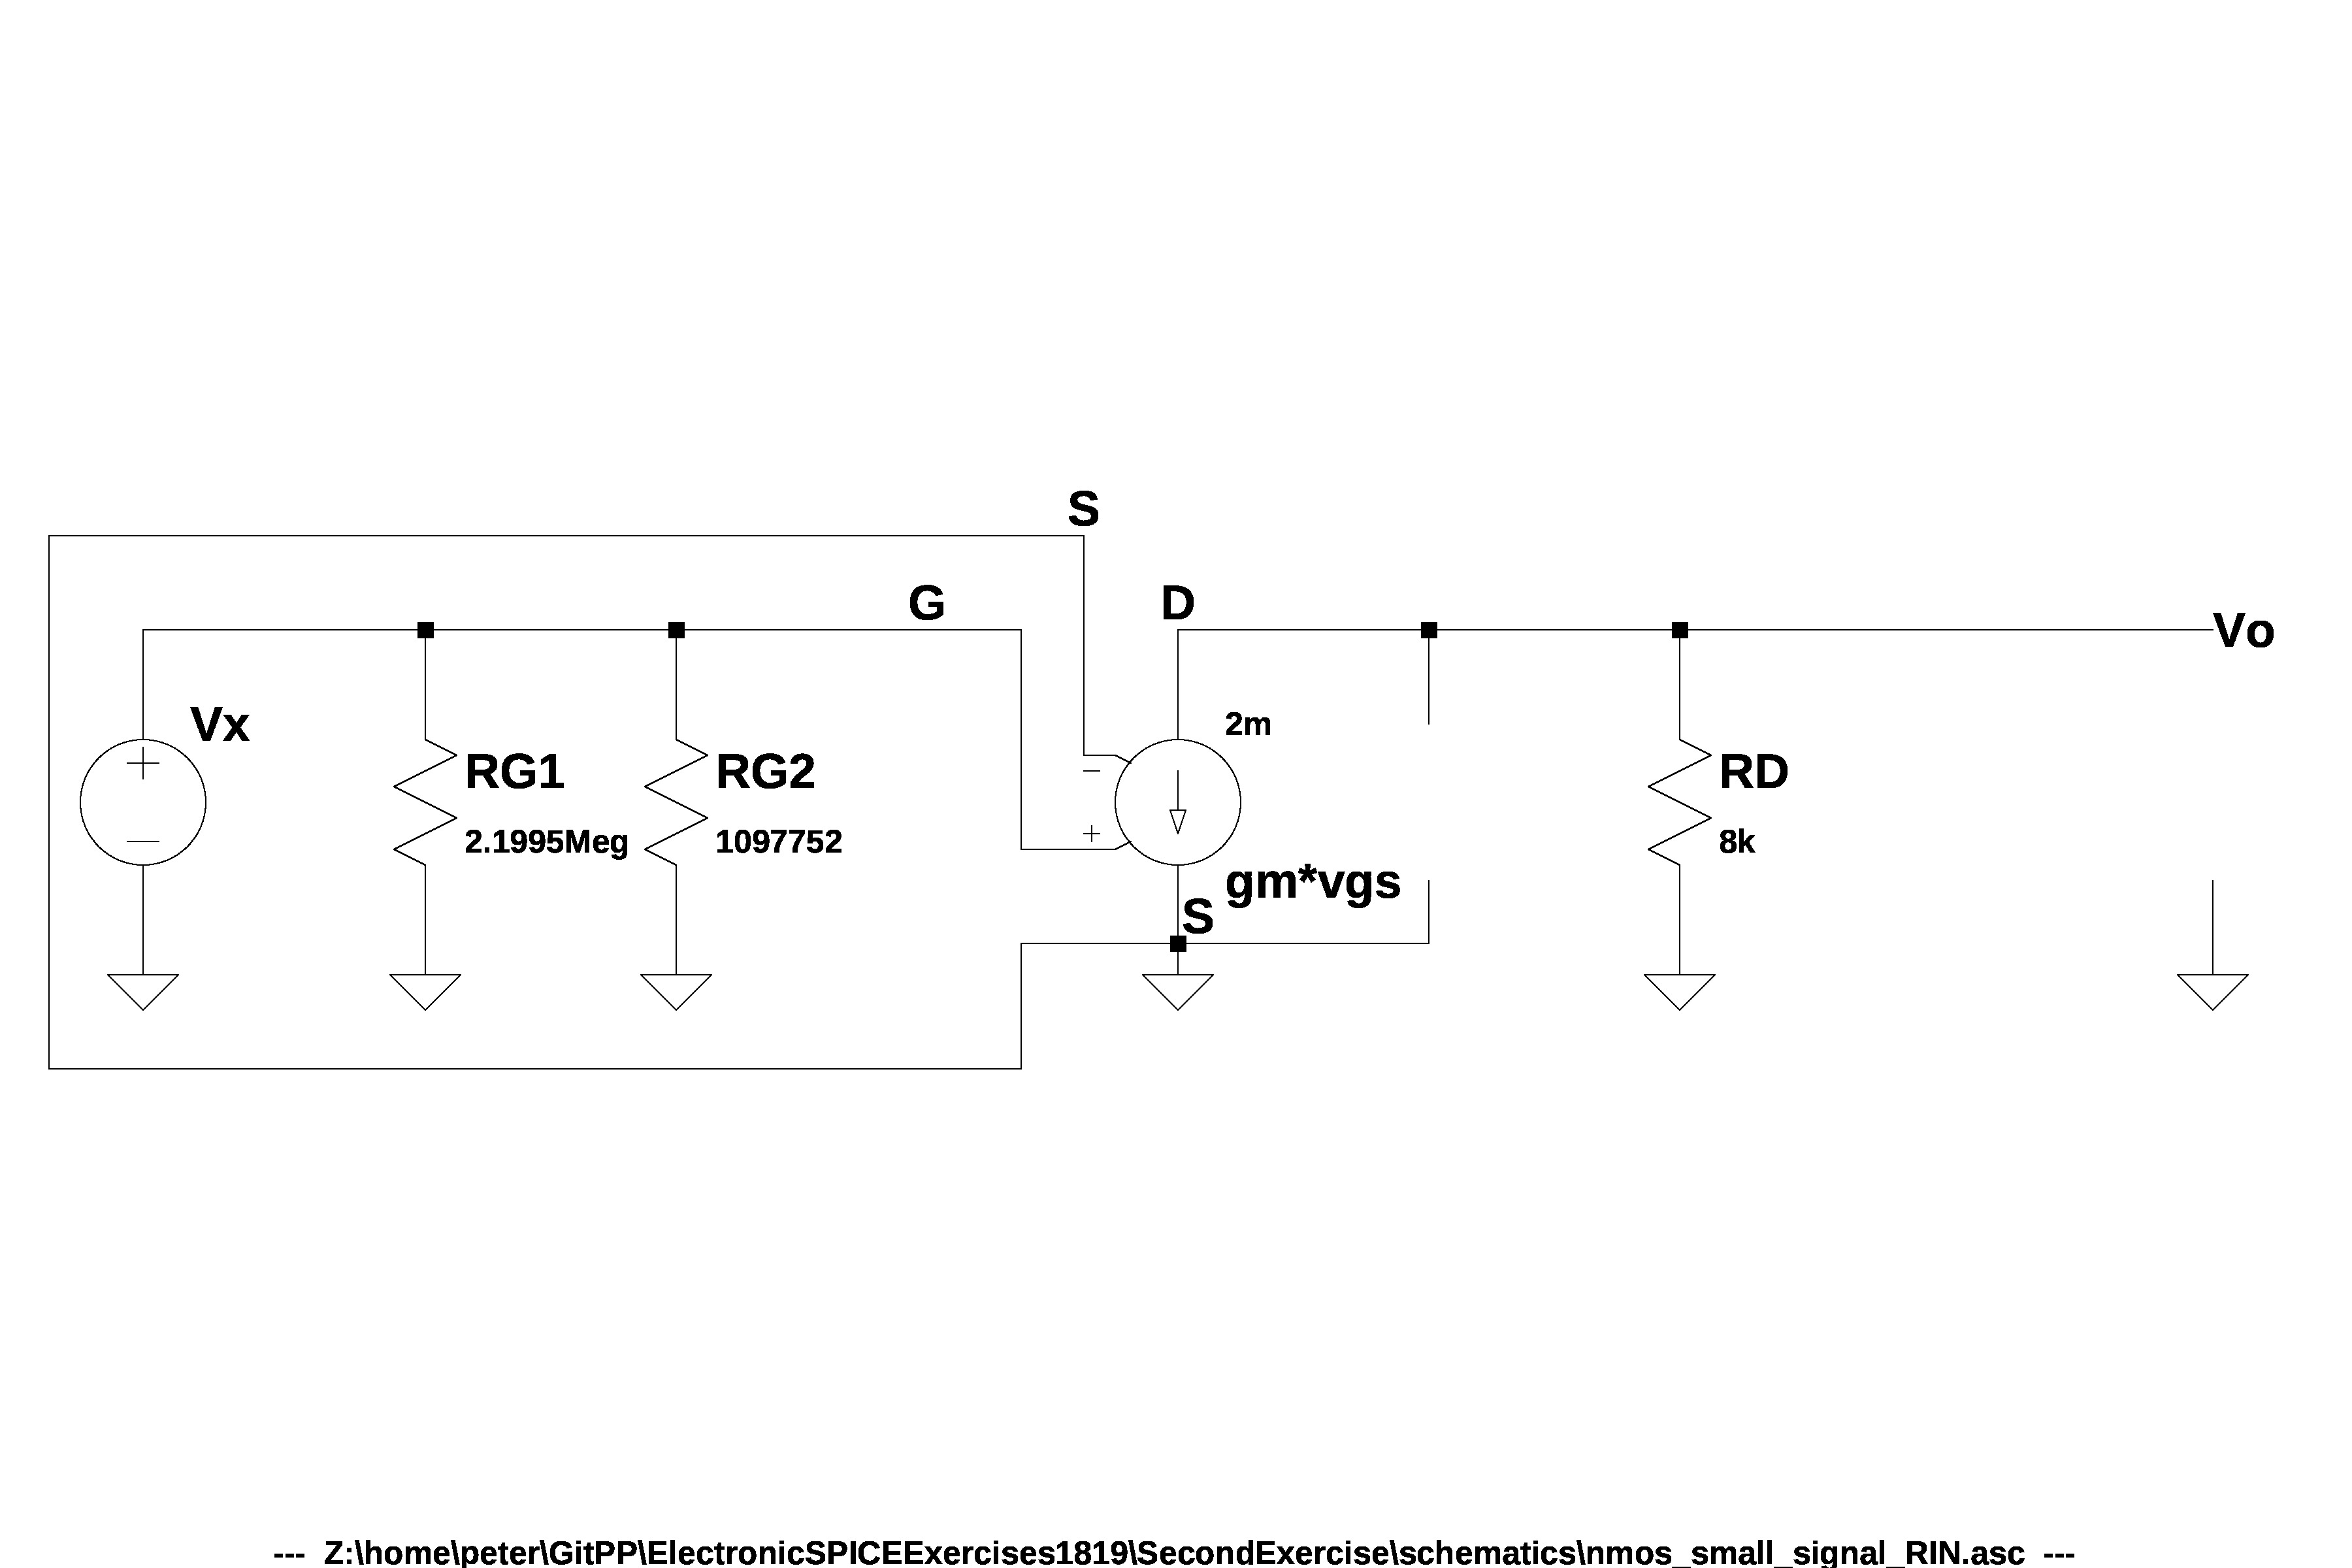
\includegraphics[width=12cm]{schematics/nmos_small_signal_RIN.jpg}
  \caption{NMOS common source amplifier - Calculating $R_{IN}$}
  \label{nmos_pi_RIN}
\end{figure}

Removing the signal, the load and applying a test voltage source as in figure \ref{nmos_pi_RIN} it is possible to calculate the input's resistance $R_{IN}$.\\

\begin{align}
R_{IN} = \frac{V_x}{I_x}\\
\end{align}
\begin{align}
I_x = \frac{V_x}{R_{G1} \parallel R_{G2}} \implies R_{G1} \parallel R_{G2} = \frac{V_x}{I_x}
\implies R_{IN} = R_{G1} \parallel R_{G2}
\end{align}
\begin{align}
R_{IN} &= \frac{R_{G1} R_{G2}}{R_{G1} + R_{G2}}\\
&= \frac{2.19550 M\Omega \cdot 1097752\Omega}{2.19550 M\Omega + 1097752\Omega}\\
&= 733.16756k\Omega \simeq 733.2k\Omega
\end{align}

\subsubsection{$R_{OUT}$ from D}\label{ROUT}

Removing the signal, the load and applying a test voltage source as in figure \ref{nmos_pi_ROUT} it is possible to calculate the output's resistance $R_{OUT}$.\\

\begin{figure}[h]
  \centering
  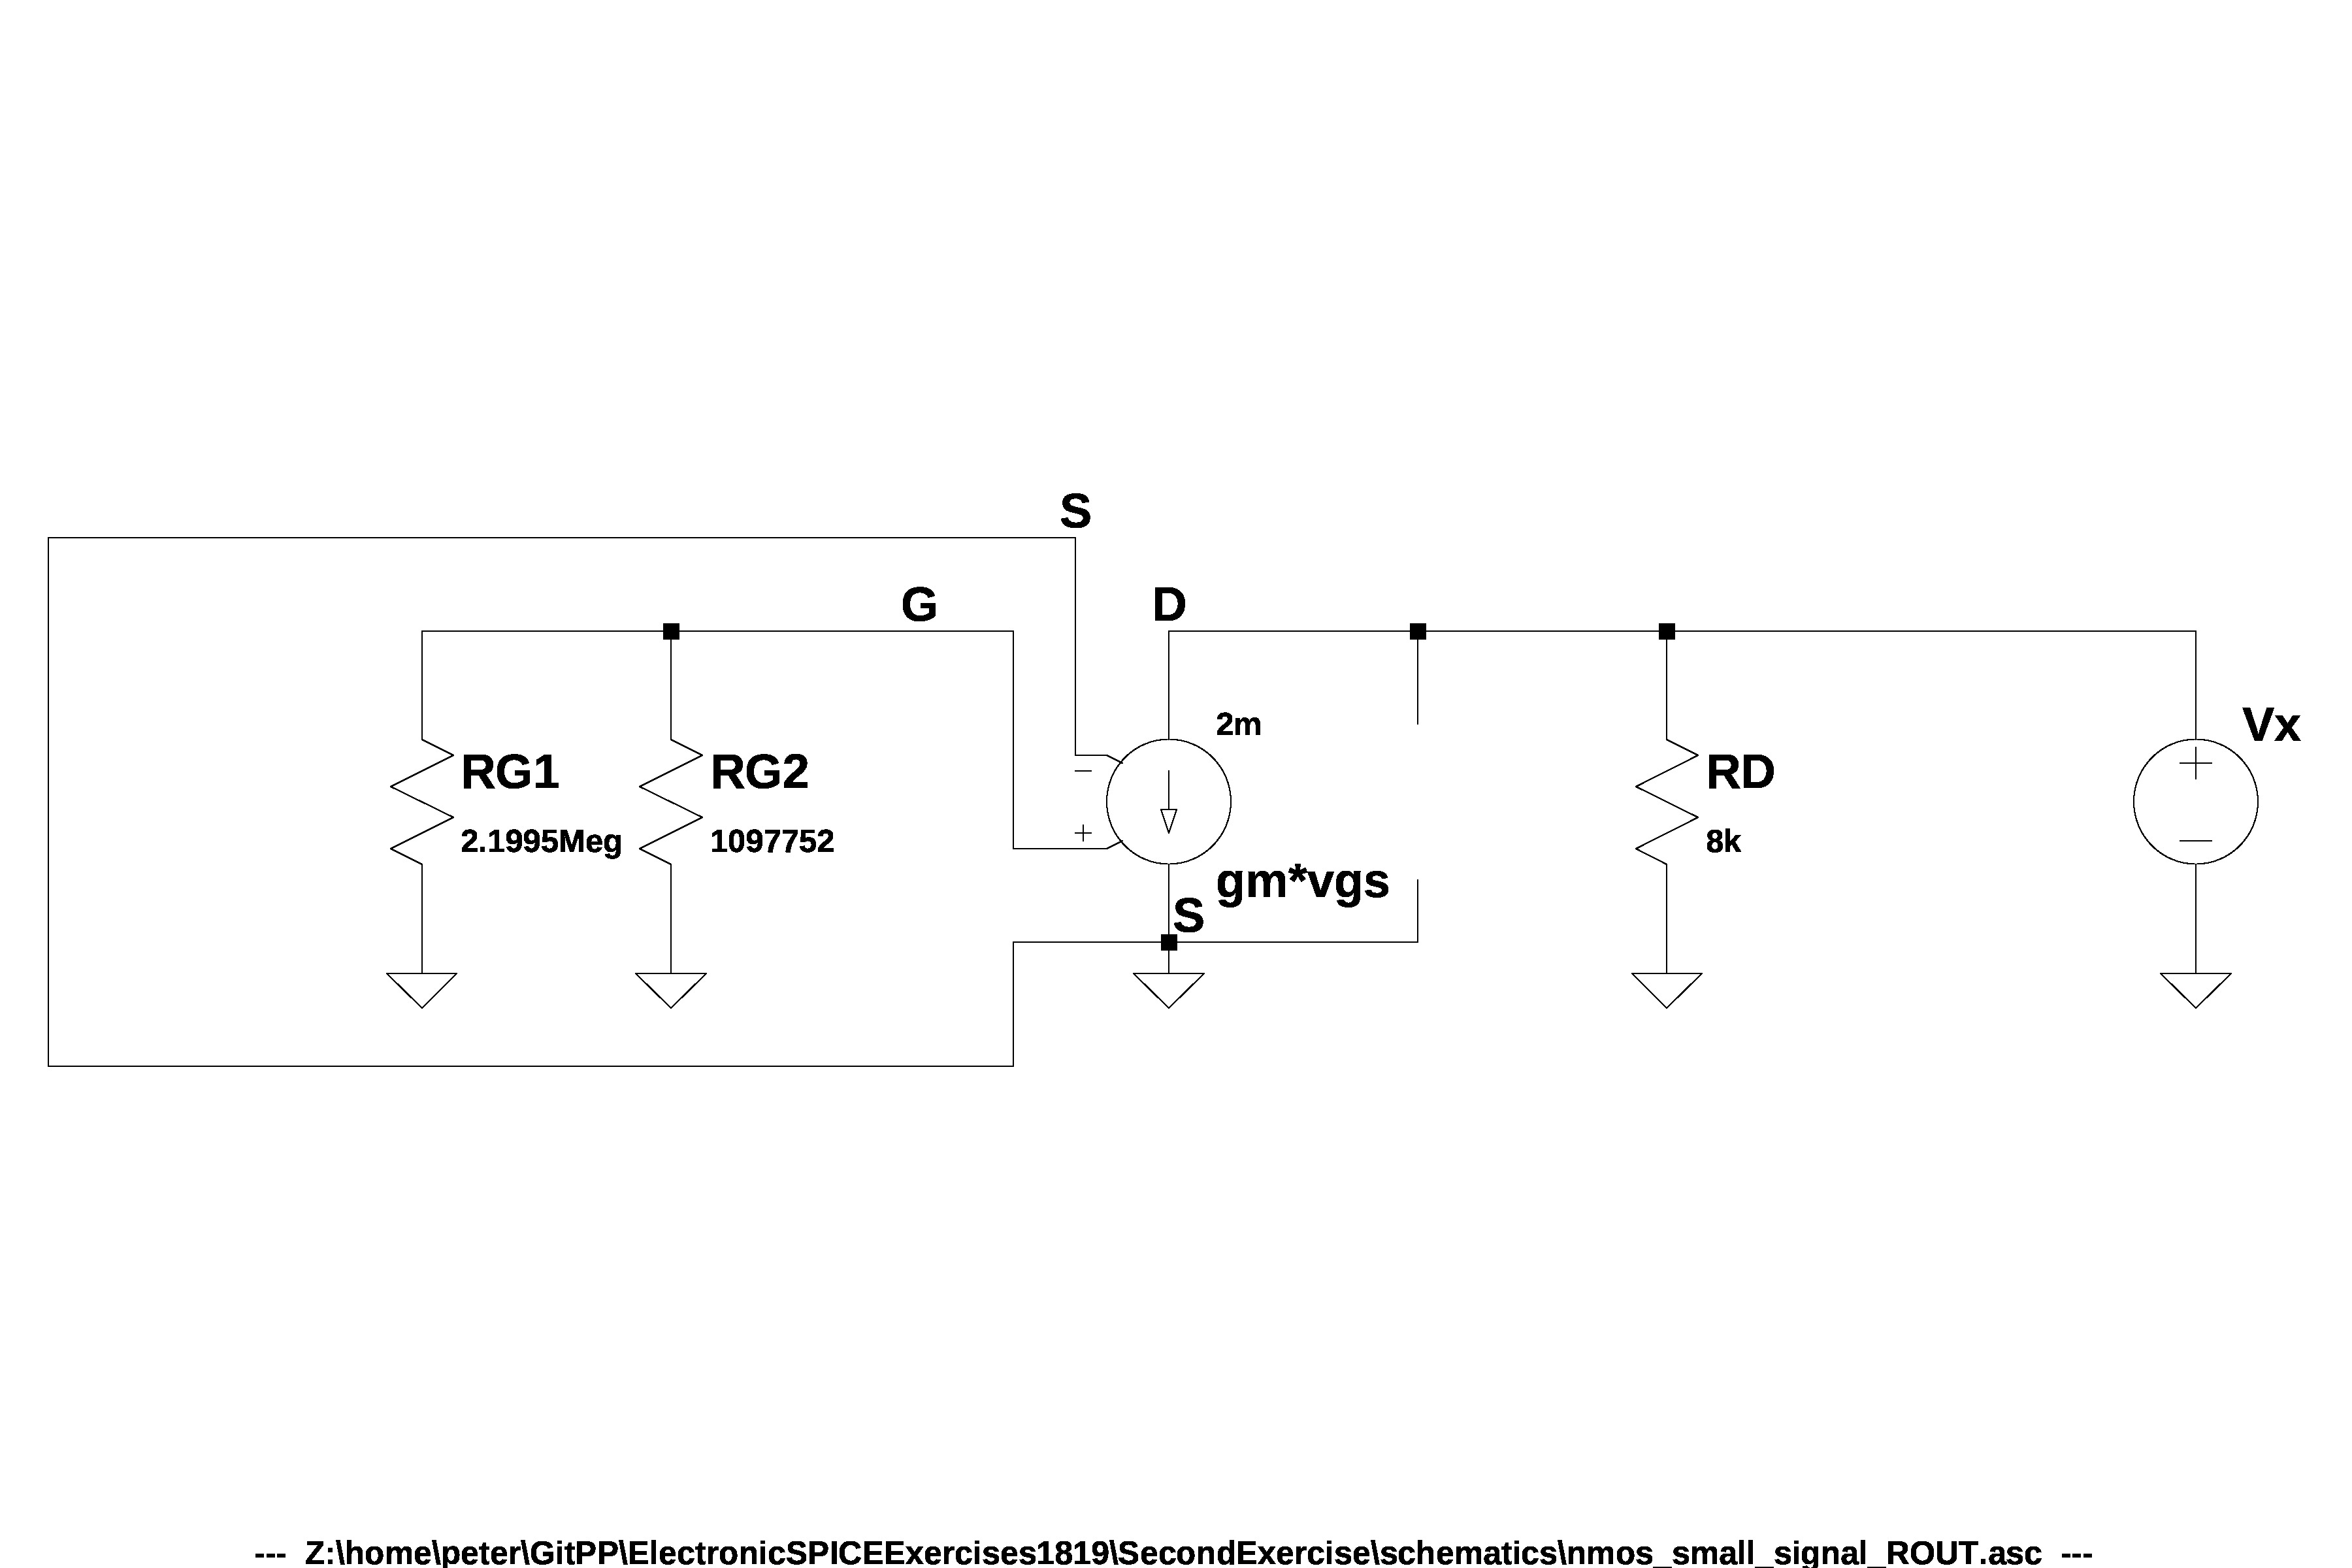
\includegraphics[width=12cm]{schematics/nmos_small_signal_ROUT.jpg}
  \caption{NMOS common source amplifier - Calculating $R_{OUT}$}
  \label{nmos_pi_ROUT}
\end{figure}

\begin{align}
R_{OUT} = \frac{V_x}{I_x}\\
\end{align}
\begin{align}
I_x = \frac{V_x}{R_D} \implies R_D = \frac{V_x}{I_x} \implies R_{OUT} = R_D 
\end{align}
\begin{align}
R_{OUT} = 8k\Omega
\end{align}

\subsubsection{Voltage Gain - without $R_{sig}$ and $R_L$}\label{AvSec}
Calculating the gain of the amplifier represented in the figure \ref{nmos_pi_gain_without_resistances}.

\begin{figure}[h]
  \centering
  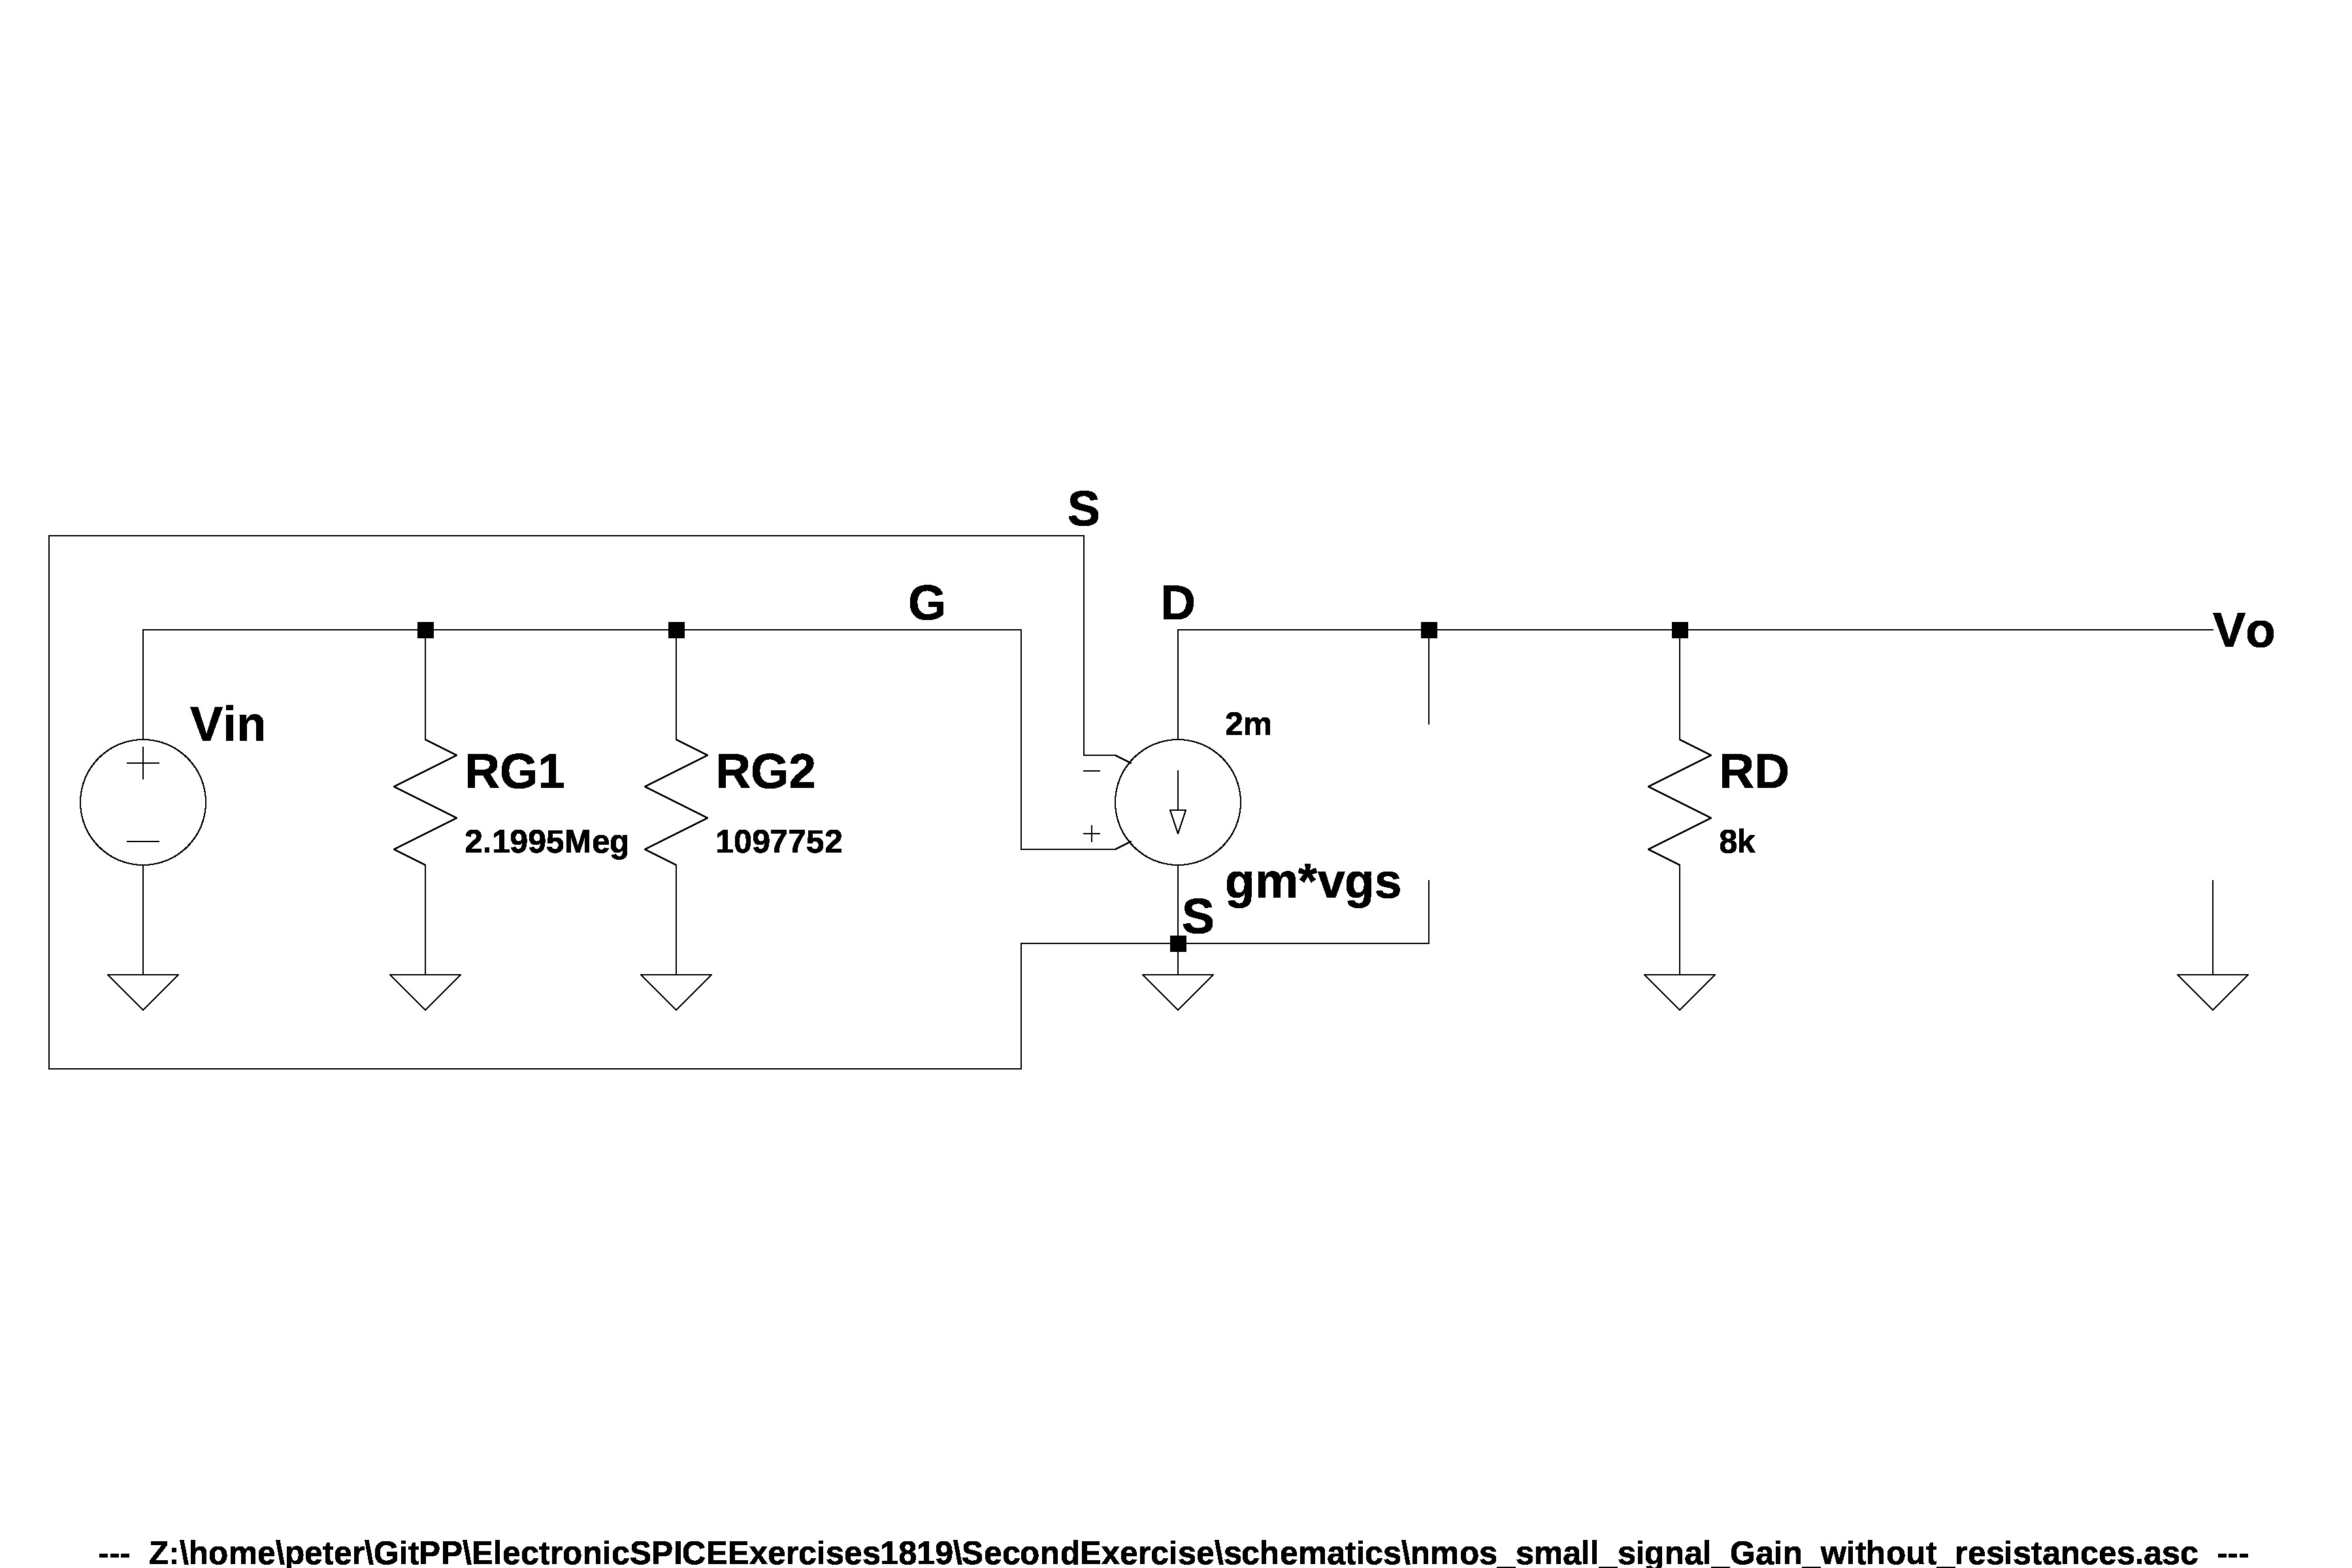
\includegraphics[width=12cm]{schematics/nmos_small_signal_without_resistances.jpg}
  \caption{NMOS common source amplifier - Calculating the voltage gain without $R_{sig}$ and $R_L$}
  \label{nmos_pi_gain_without_resistances}
\end{figure}

\begin{align}
v_{in} = v_{gs}\\
v_{o} = - g_m v_{gs} R_D
\end{align}

\begin{align}
A_v = \frac{v_o}{v_{in}} = \frac{- g_m v_{gs} R_D}{v_{gs}} = - g_m R_D = 2mA/V \cdot 8k\Omega = -16 \quad V/V \label{Av}
\end{align}

\subsubsection{Voltage Gain - with $R_{sig}$ and $R_L$}\label{GvSec}
Calculating the gain of the amplifier represented in the figure \ref{nmos_pi_gain_with_resistances}.

\begin{figure}[h]
  \centering
  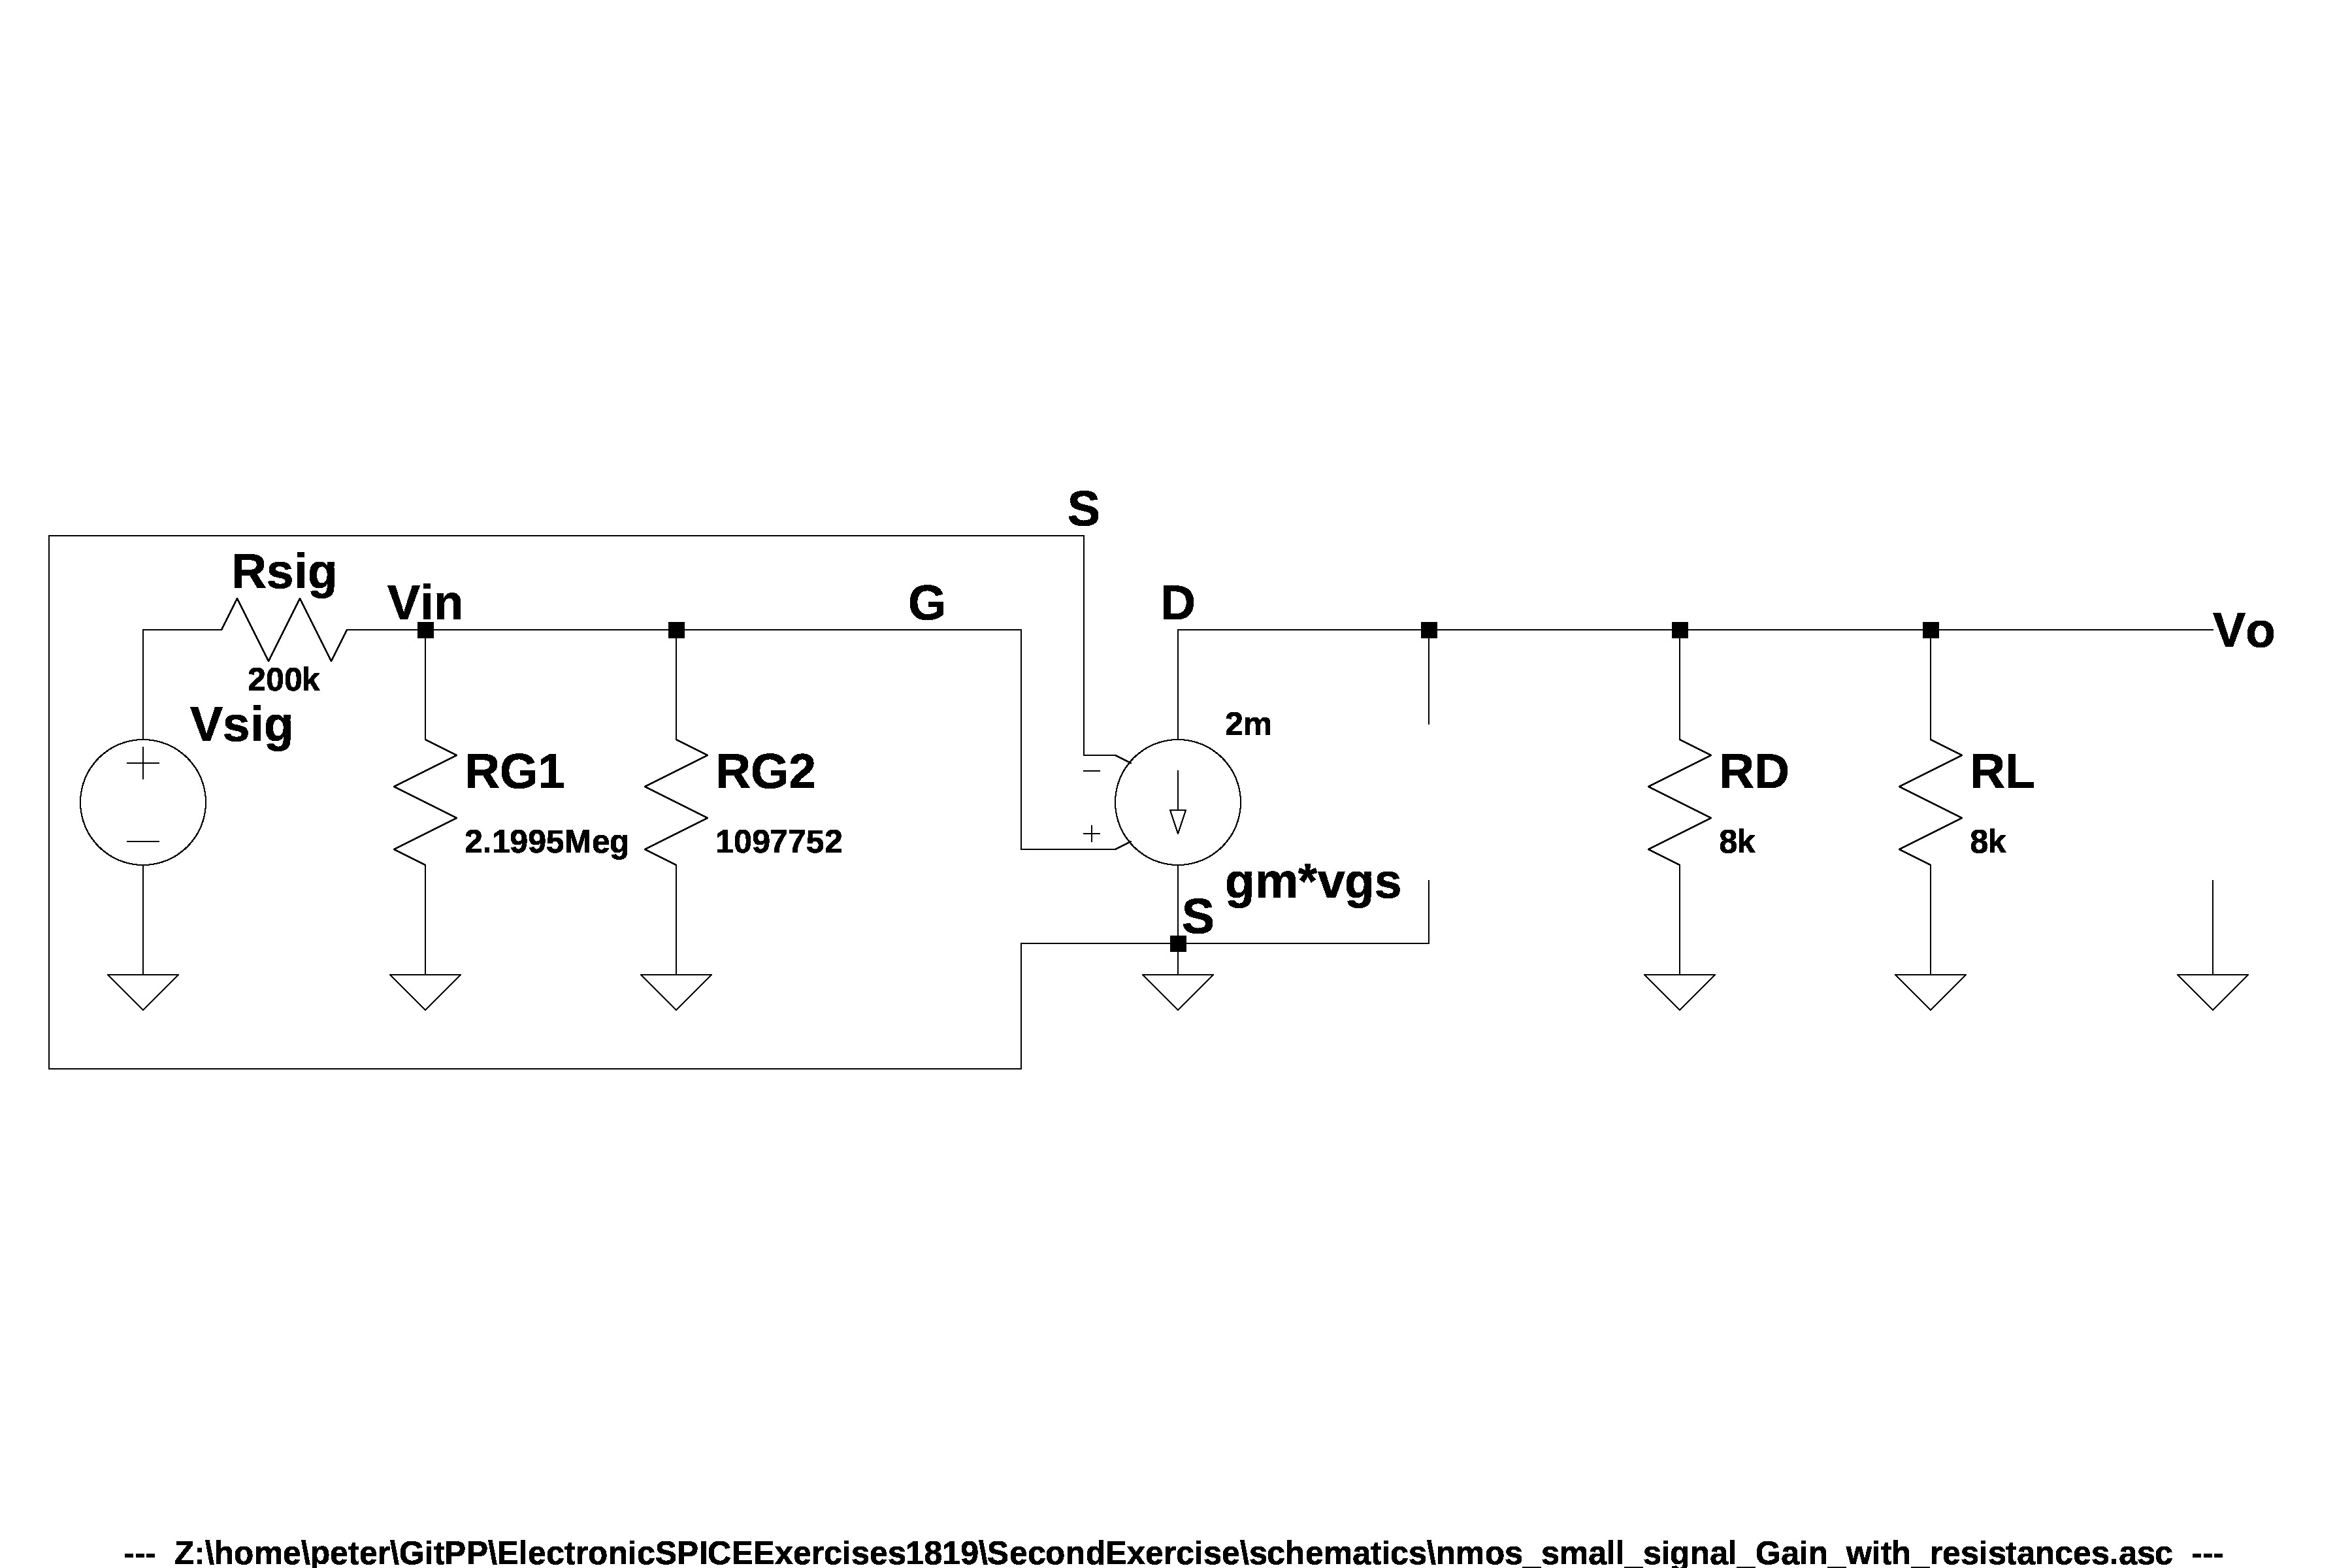
\includegraphics[width=12cm]{schematics/nmos_small_signal_with_resistances.jpg}
  \caption{NMOS common source amplifier - Calculating the voltage gain with $R_{sig}$ and $R_L$}
  \label{nmos_pi_gain_with_resistances}
\end{figure}

\begin{align}
I_{sig} &= \frac{v_{sig}}{R_{sig} + (R_{G1} \parallel R_{G2})}
\end{align}

\begin{align}
v_{in} = v_{gs} &= v_{sig} - R_{sig} I_{sig}\\
&= v_{sig} - R_{sig} \frac{v_{sig}}{R_{sig} + (R_{G1} \parallel R_{G2})}\\
&= v_{sig} \left(1 - R_{sig} \frac{1}{R_{sig} + (R_{G1} \parallel R_{G2})}\right)
\end{align}

\begin{align}
v_o &= -g_m v_{gs} (R_D \parallel R_L)\\
&= -g_m v_{sig} \left(1 - R_{sig} \frac{1}{R_{sig} + (R_{G1} \parallel R_{G2})}\right) (R_D \parallel R_L)
\end{align}


\begin{align}
G_v = \frac{v_o}{v_{sig}} &= \frac{-g_m v_{sig} \left(1 - R_{sig} \frac{1}{R_{sig} + (R_{G1} \parallel R_{G2})}\right) (R_D \parallel R_L)}{v_{sig}}\\
&= -g_m \left(1 - R_{sig} \frac{1}{R_{sig} + (R_{G1} \parallel R_{G2})}\right) (R_D \parallel R_L)\\
&= -g_m \left(1 - R_{sig} \frac{1}{R_{sig} + \left(\frac{R_{G1}R_{G2}}{R_{G1}+R_{G2}}\right)}\right) \left(\frac{R_{D}R_{L}}{R_{D}+R_{L}}\right)\\
&= - 2mA/V \left(1 - 200k\Omega \frac{1}{200k\Omega + \left(\frac{2.19550M\Omega \cdot 1097752\Omega}{2.19550M\Omega +1097752\Omega}\right)}\right) \left(\frac{8k\Omega \cdot 8k\Omega}{8k\Omega + 8k\Omega}\right)\\
&= -6.28296 \quad V/V \simeq -6.3 \quad V/V \label{Gv}
\end{align}

\clearpage
\section{SPICE simulations}
\subsection{DC simulation - Operating Point}\label{DCsim}
\lstinputlisting{netlist/a.cir}
The results confirm the DC analysis (results calculated in the section \ref{DCsec}).
\lstinputlisting{netlist/a.op}

\subsection{AC simulation - $Av$, $R_{IN}$ and $R_{OUT}$}
\lstinputlisting{netlist/nmos_small_signal_RIN_ROUT.cir}
The result confirm the analysis (result calculated in the section \ref{AvSec}, expression \ref{Av}).
\lstinputlisting{netlist/nmos_small_signal_RIN_ROUT.tf}

\subsection{AC simulation - $Gv$}
\lstinputlisting{netlist/nmos_small_signal_RIN_ROUT_with_Rs_Rl.cir}
The result confirm the analysis (result calculated in the section \ref{GvSec}, expression \ref{Gv}).
\lstinputlisting{netlist/nmos_small_signal_RIN_ROUT_with_Rs_Rl.tf}

\chapter{NMOS common source amplifier without bypass capacitance}
\begin{figure}[h]
  \centering
  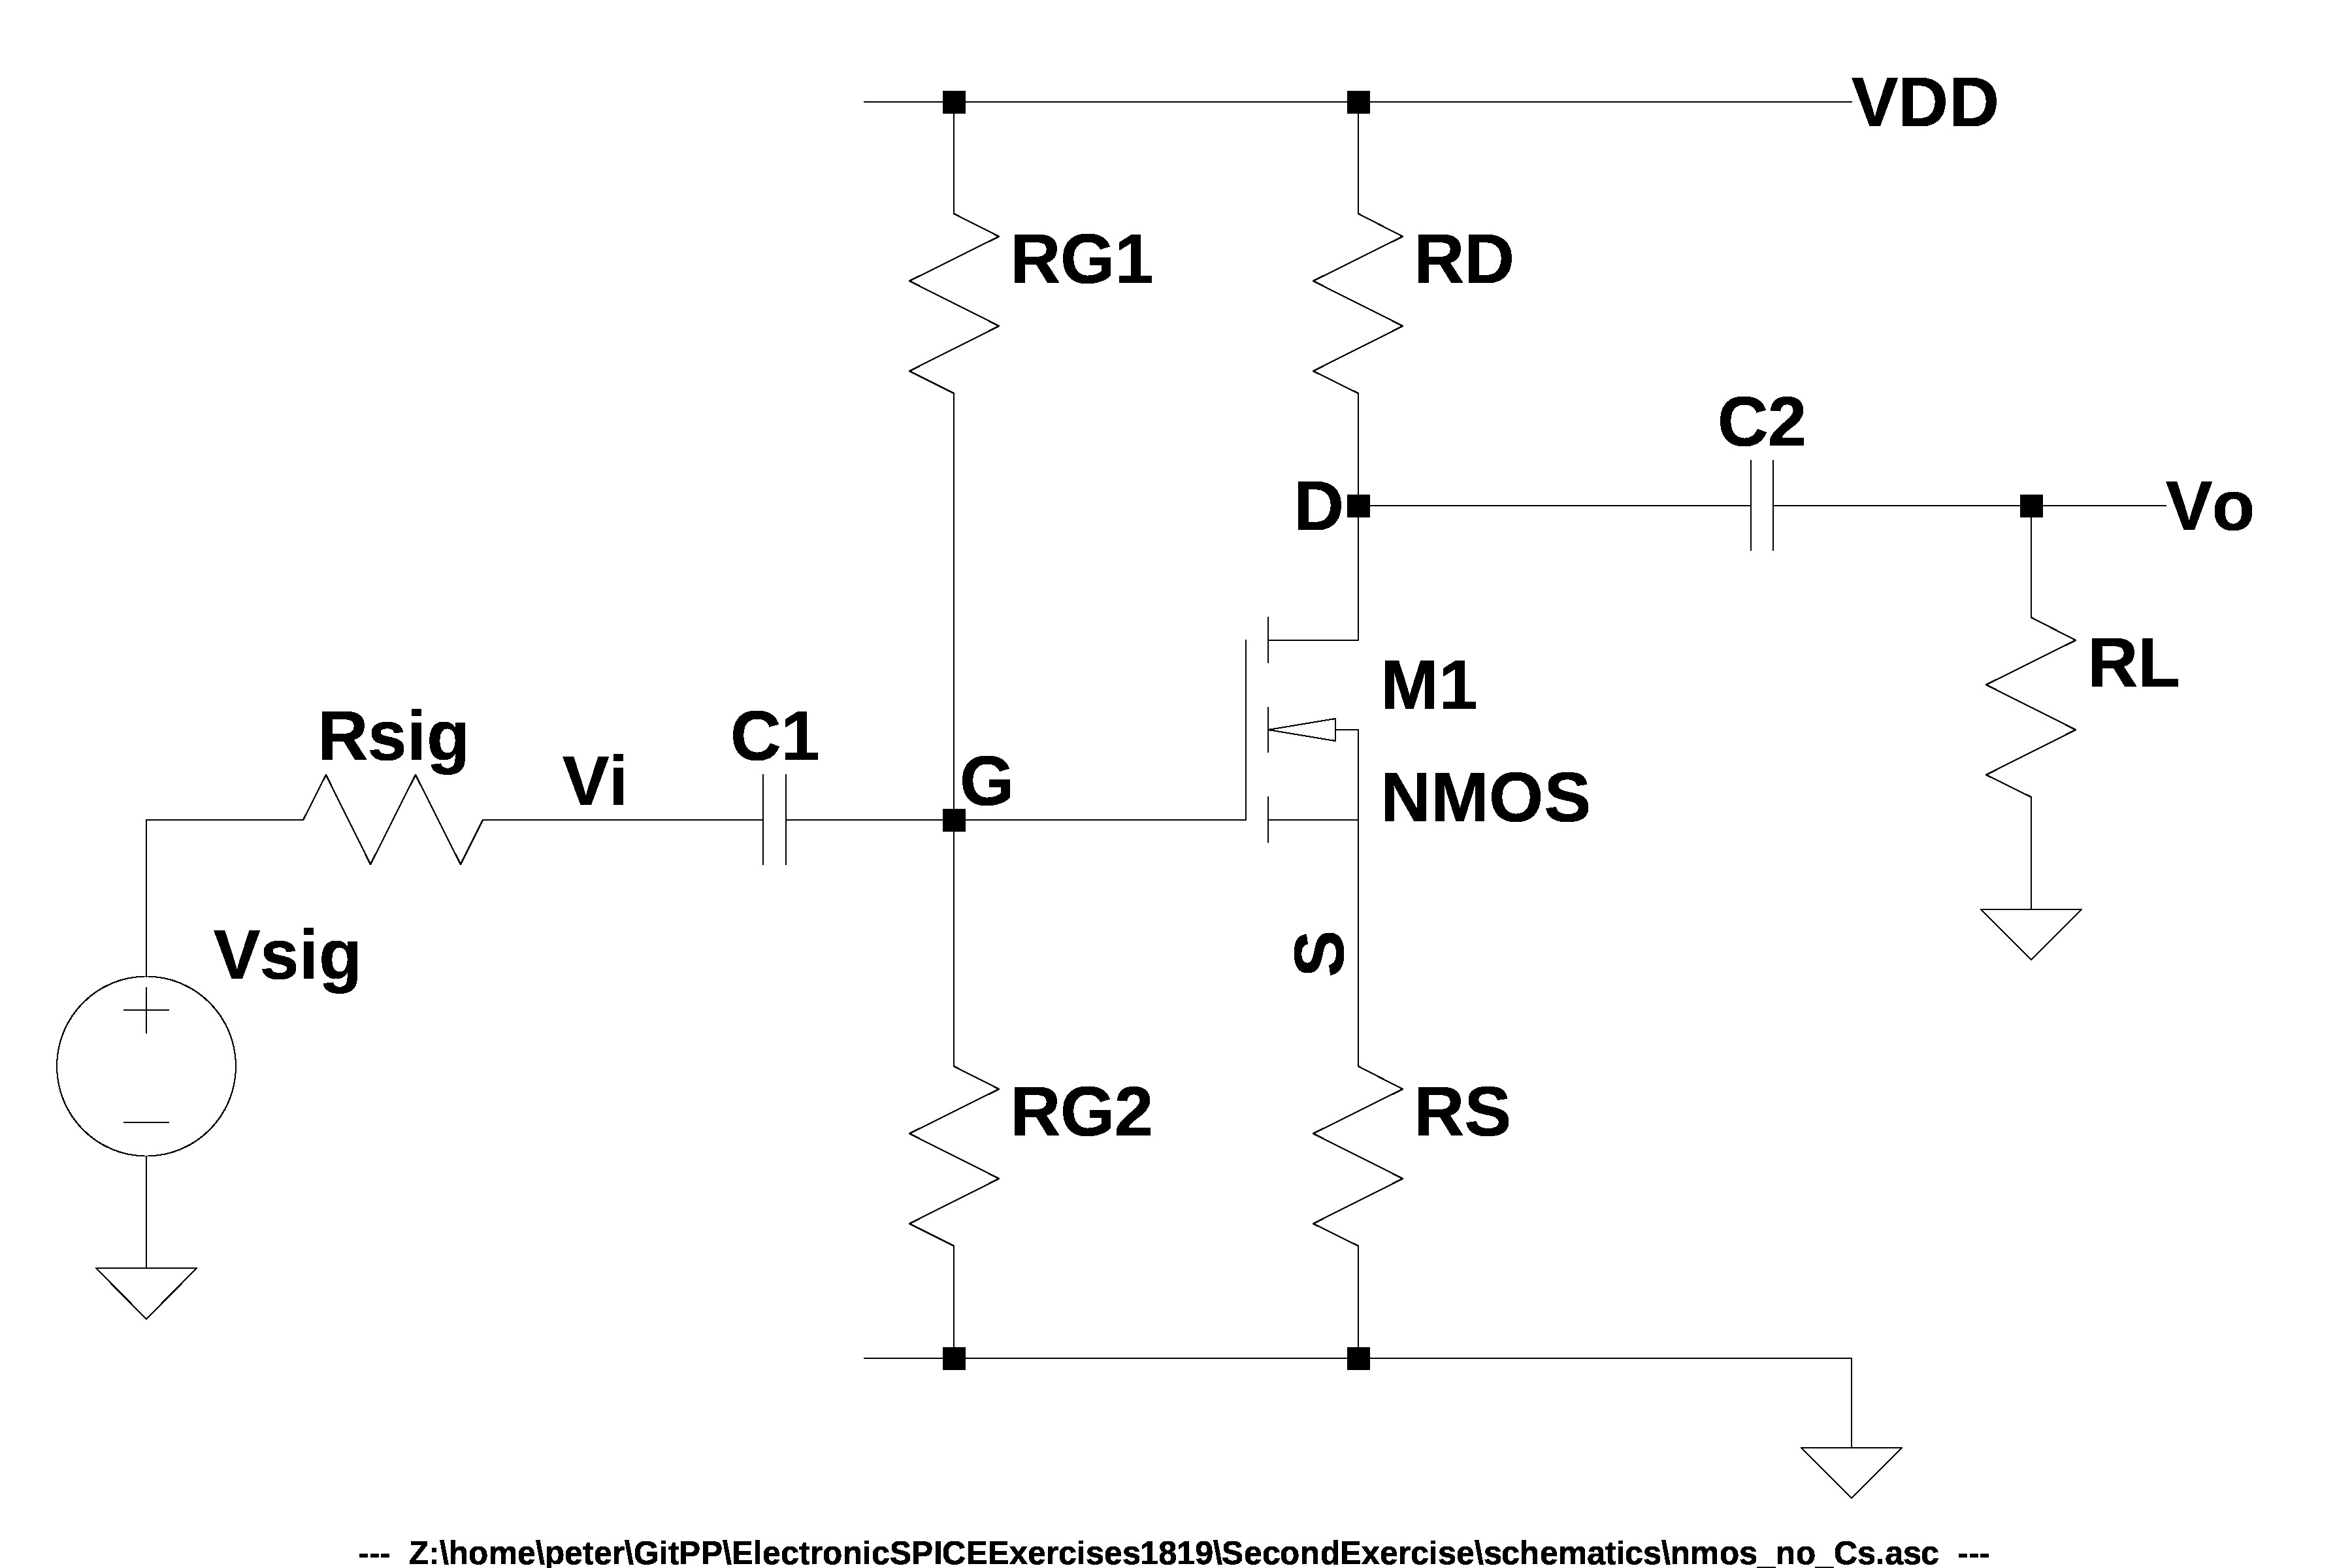
\includegraphics[width=12cm]{schematics/nmos_no_Cs.jpg}
  \caption{NMOS common source amplifier}
  \label{nmos_no_Cs}
\end{figure}

Designing the common source amplifier of the figure \ref{nmos_no_Cs} .\\
The MOSFET should have a $V_t = 1V$, a $K_n = 4mA/V$ and a $\lambda = 0$.\\
Other requested parameters are: $I_{DQ} = 0.5mA$, $V_S = 3.5V$, $V_D = 11V$, $V_{DD} = 15V$ and $R_{G2} = 1097752\Omega$.\par

\section{Analytic solution}
The figure \ref{nmos_DC_no_Cs} represents the circuit for the DC analysis.\\
It is the same circuit analysed on the section \ref{nmos_DC_section} and so the results of that section are considered also for this section.\par

\begin{figure}[h]
  \centering
  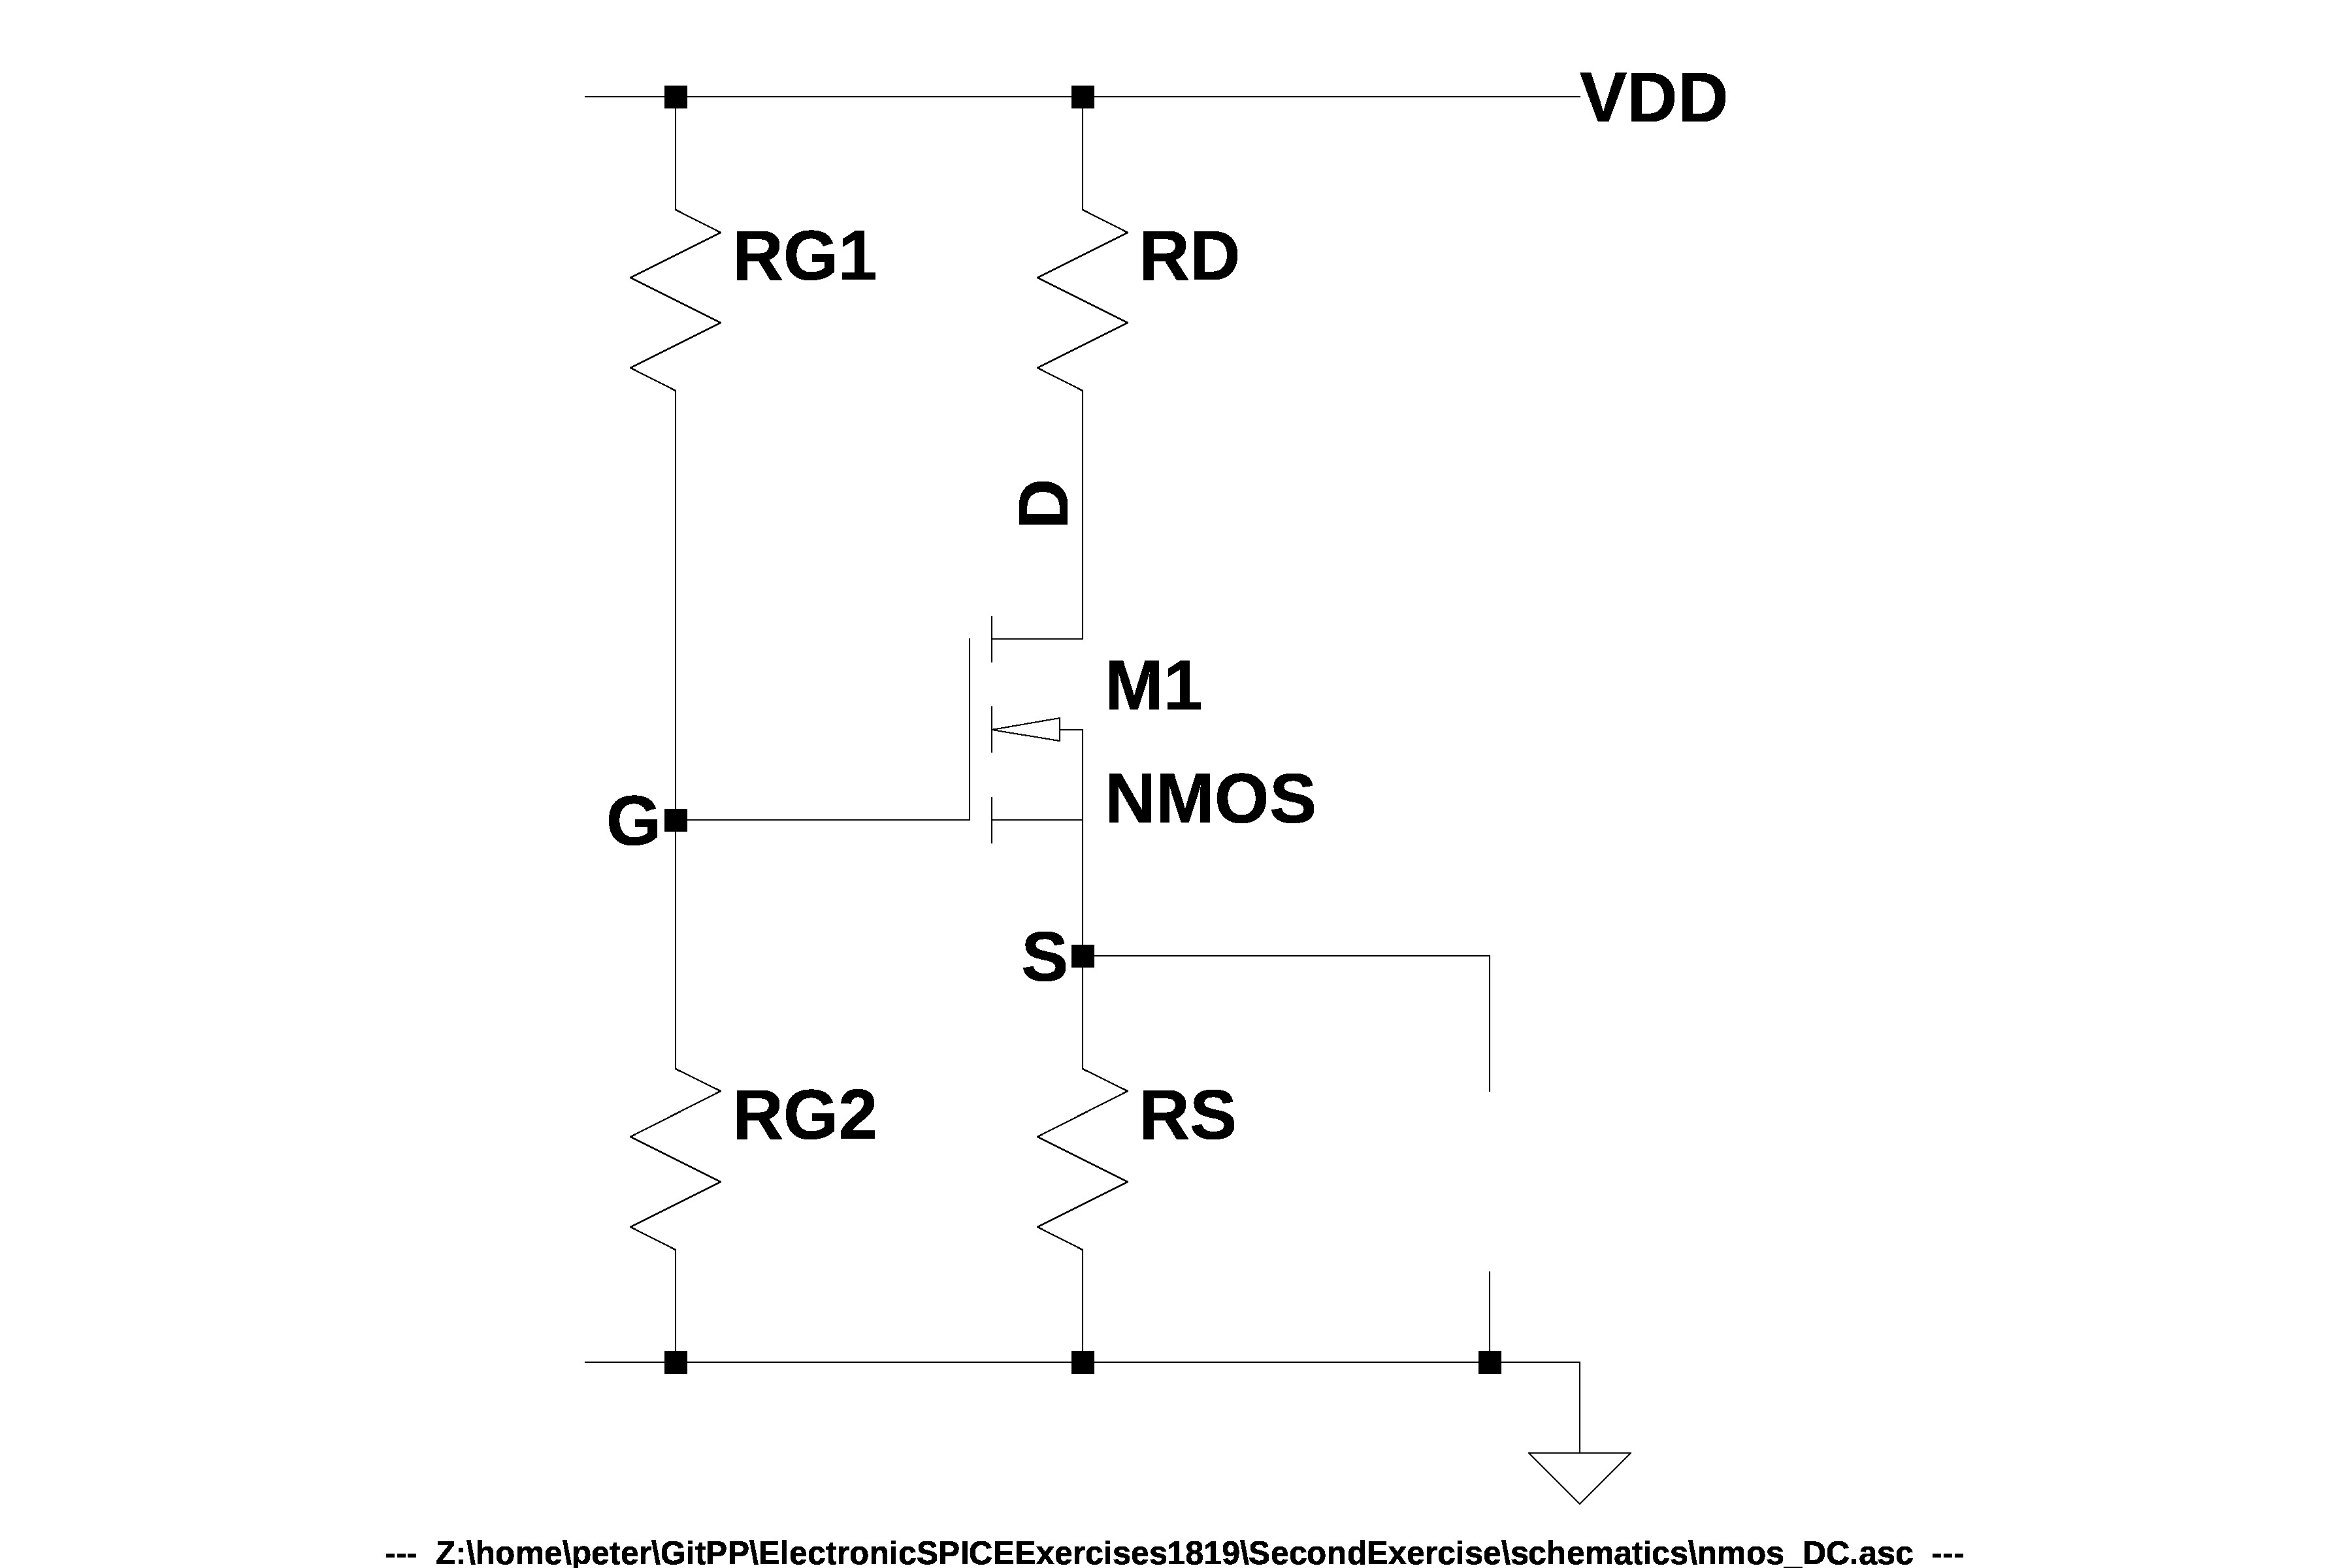
\includegraphics[width=12cm]{schematics/nmos_DC.jpg}
  \caption{NMOS common source amplifier - DC analysis}
  \label{nmos_DC_no_Cs}
\end{figure}

\subsubsection{Hybrid $\pi$ model}
In this case it is used the hybrid $\pi$ model (figure \ref{nmos_pi_no_Cs}).\par

\begin{figure}[h]
  \centering
  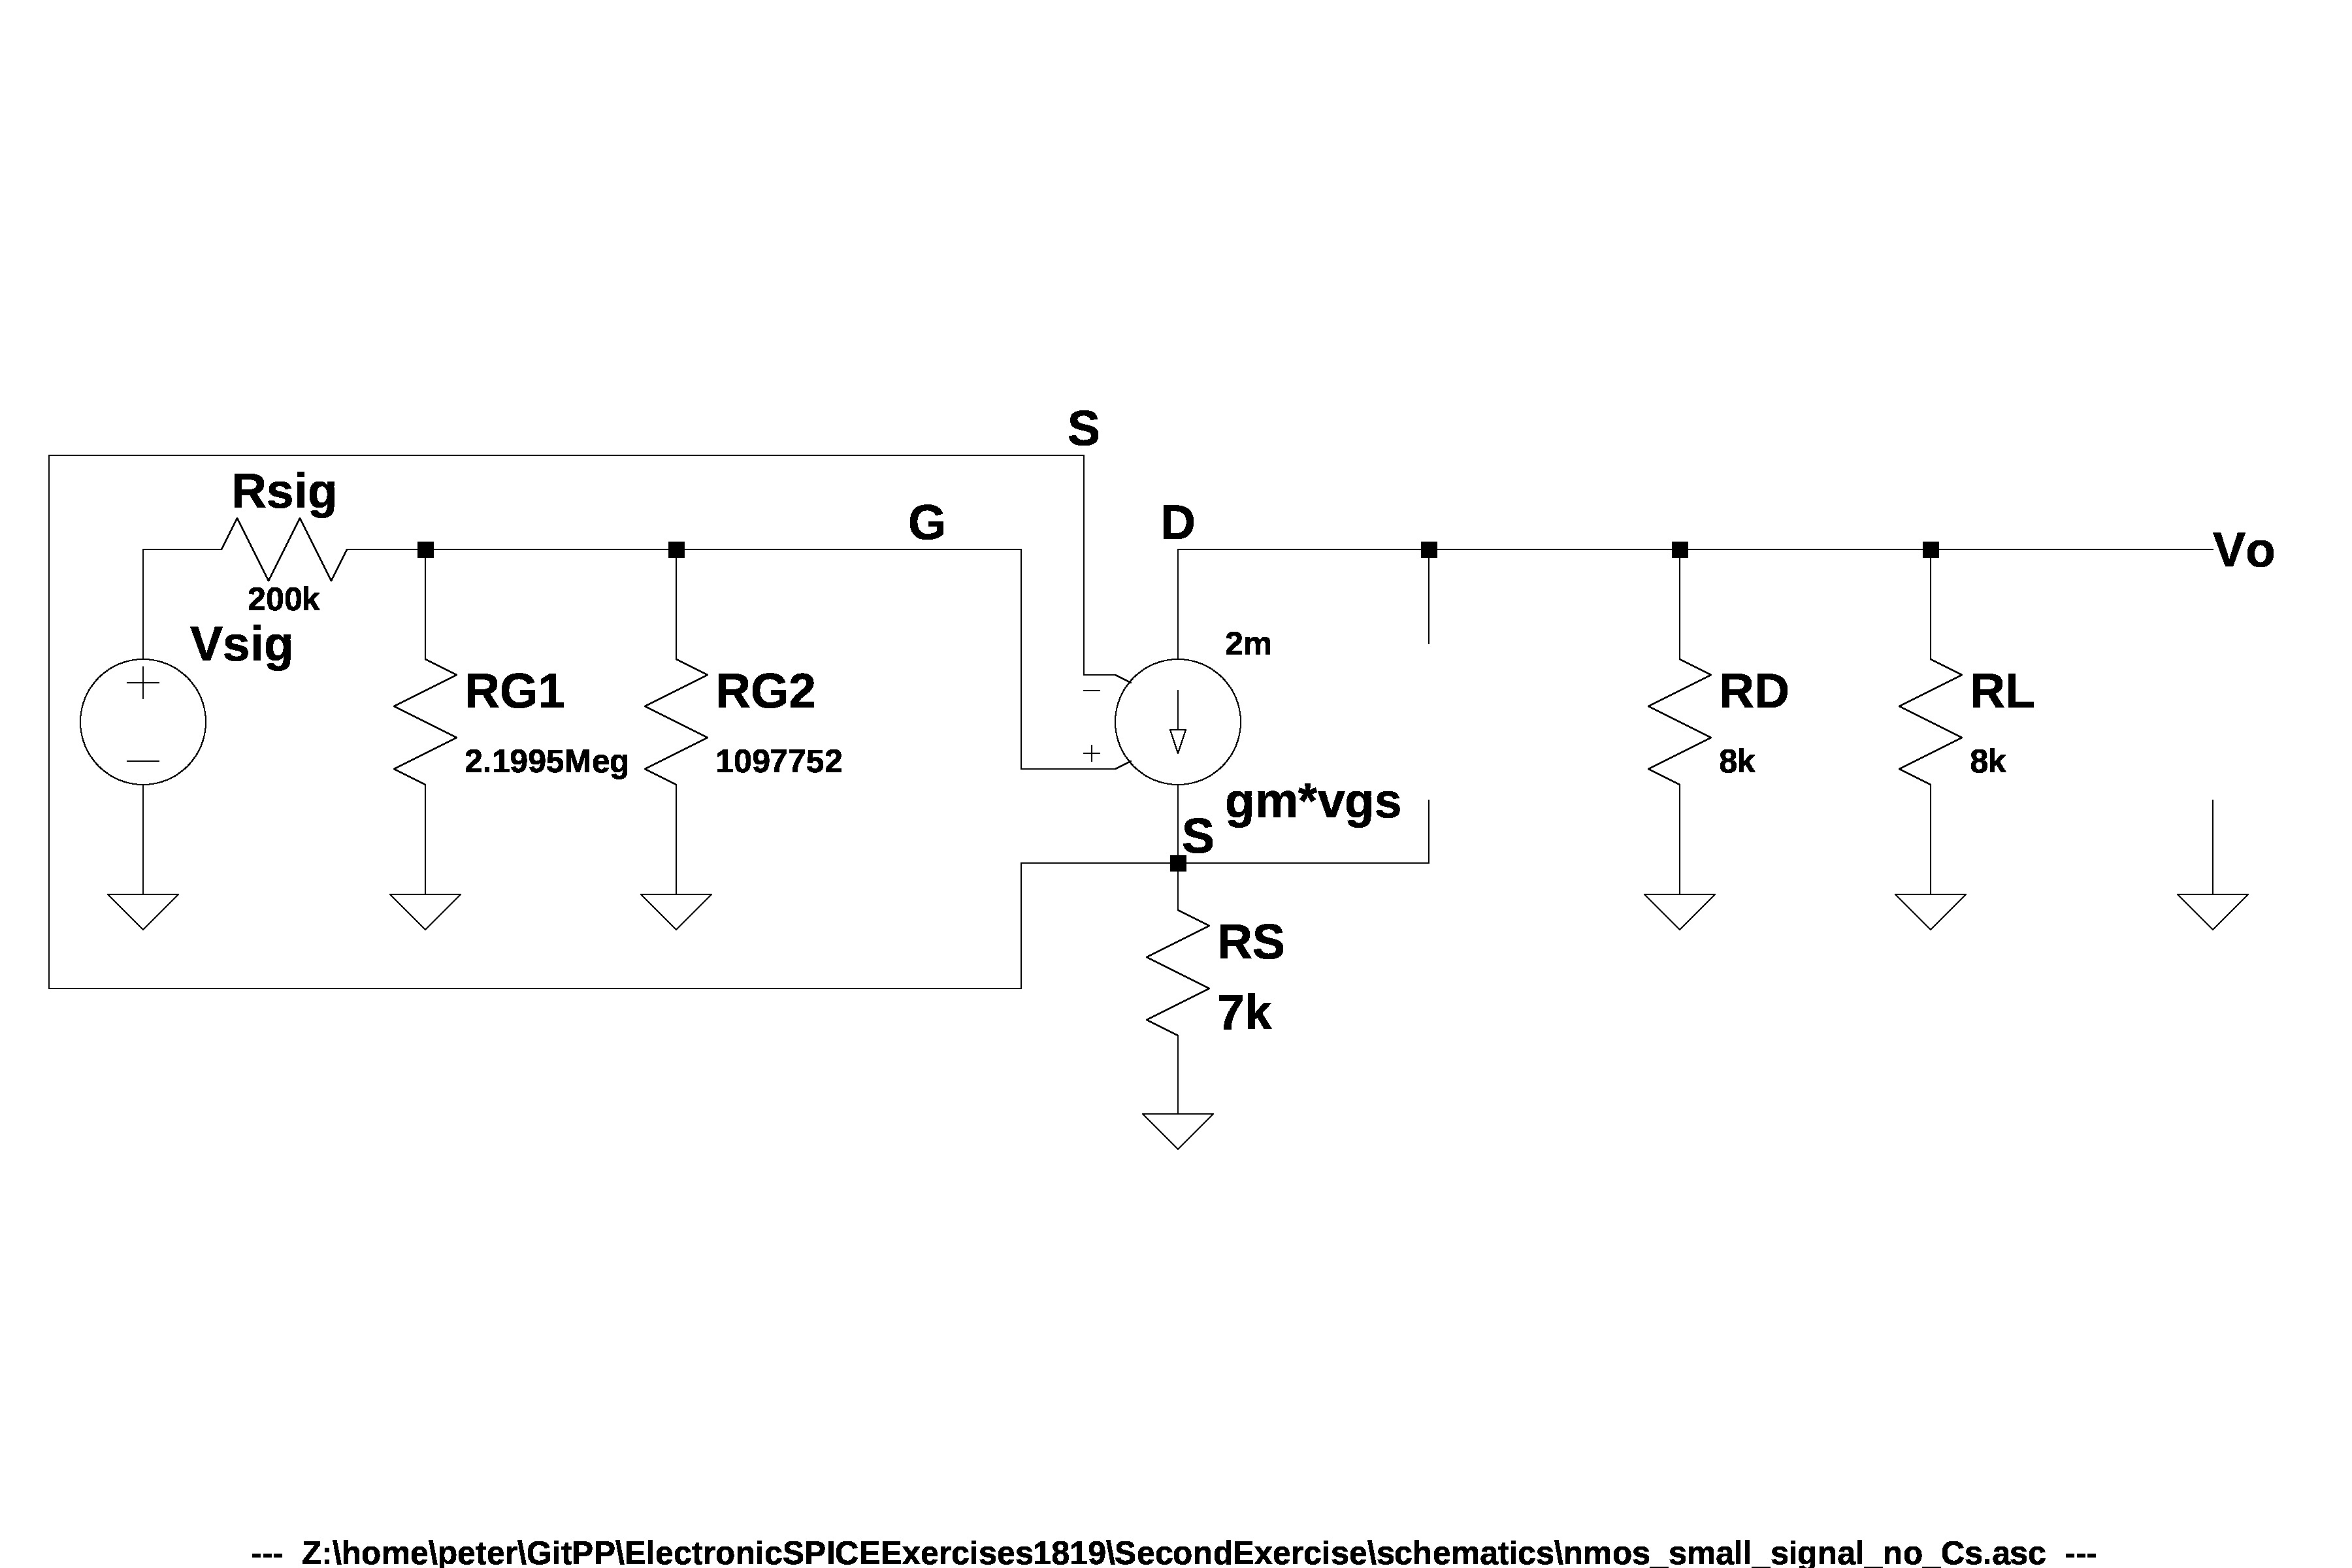
\includegraphics[width=12cm]{schematics/nmos_small_signal_no_Cs.jpg}
  \caption{NMOS common source amplifier - Hybrid $\pi$ model}
  \label{nmos_pi_no_Cs}
\end{figure}

\subsubsection{$R_{IN}$ from $G$}

\begin{figure}[h]
  \centering
  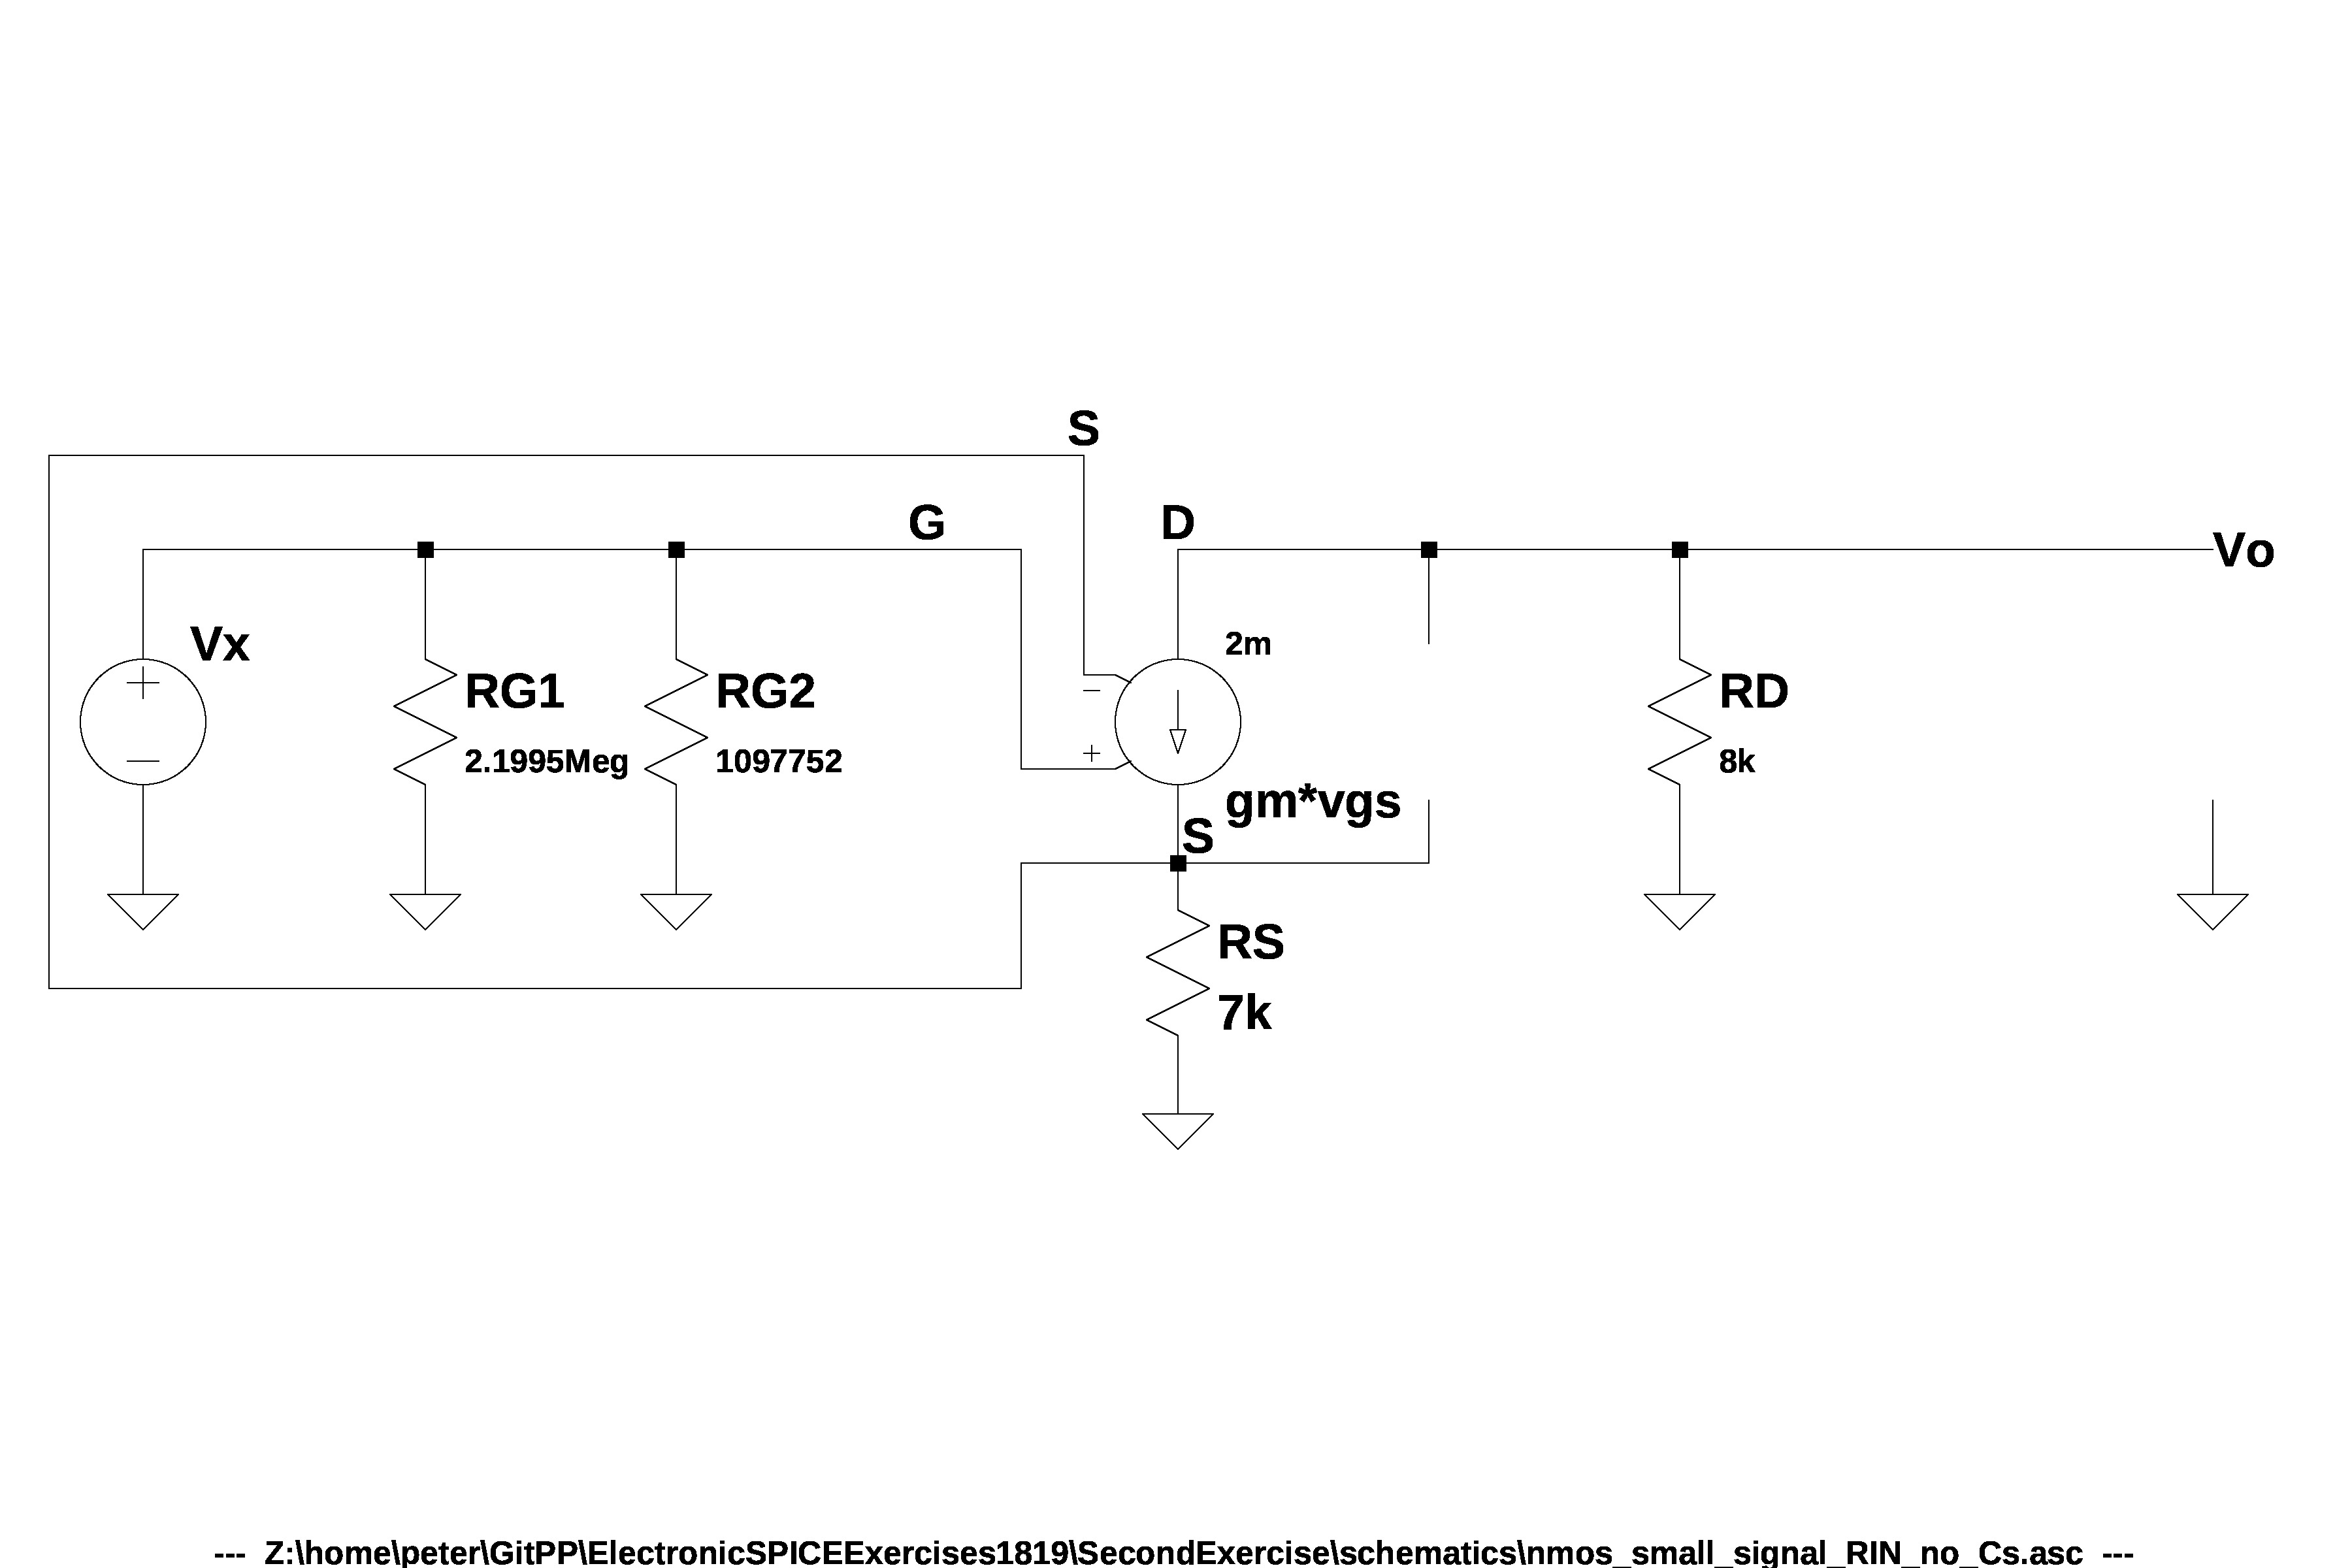
\includegraphics[width=12cm]{schematics/nmos_small_signal_RIN_no_Cs.jpg}
  \caption{NMOS common source amplifier - Calculating $R_{IN}$}
  \label{nmos_pi_RIN_no_Cs}
\end{figure}

Removing the signal, the load and applying a test voltage source as in figure \ref{nmos_pi_RIN_no_Cs} it is possible to calculate the input's resistance $R_{IN}$.\\
The result is obviously equal to the section \ref{RIN}'s result.\par

\subsubsection{$R_{OUT}$ from D}

Removing the signal, the load and applying a test voltage source as in figure \ref{nmos_pi_ROUT_no_Cs} it is possible to calculate the output's resistance $R_{OUT}$.\\
The result is equal to the section \ref{ROUT}'s result.\par

\begin{figure}[h]
  \centering
  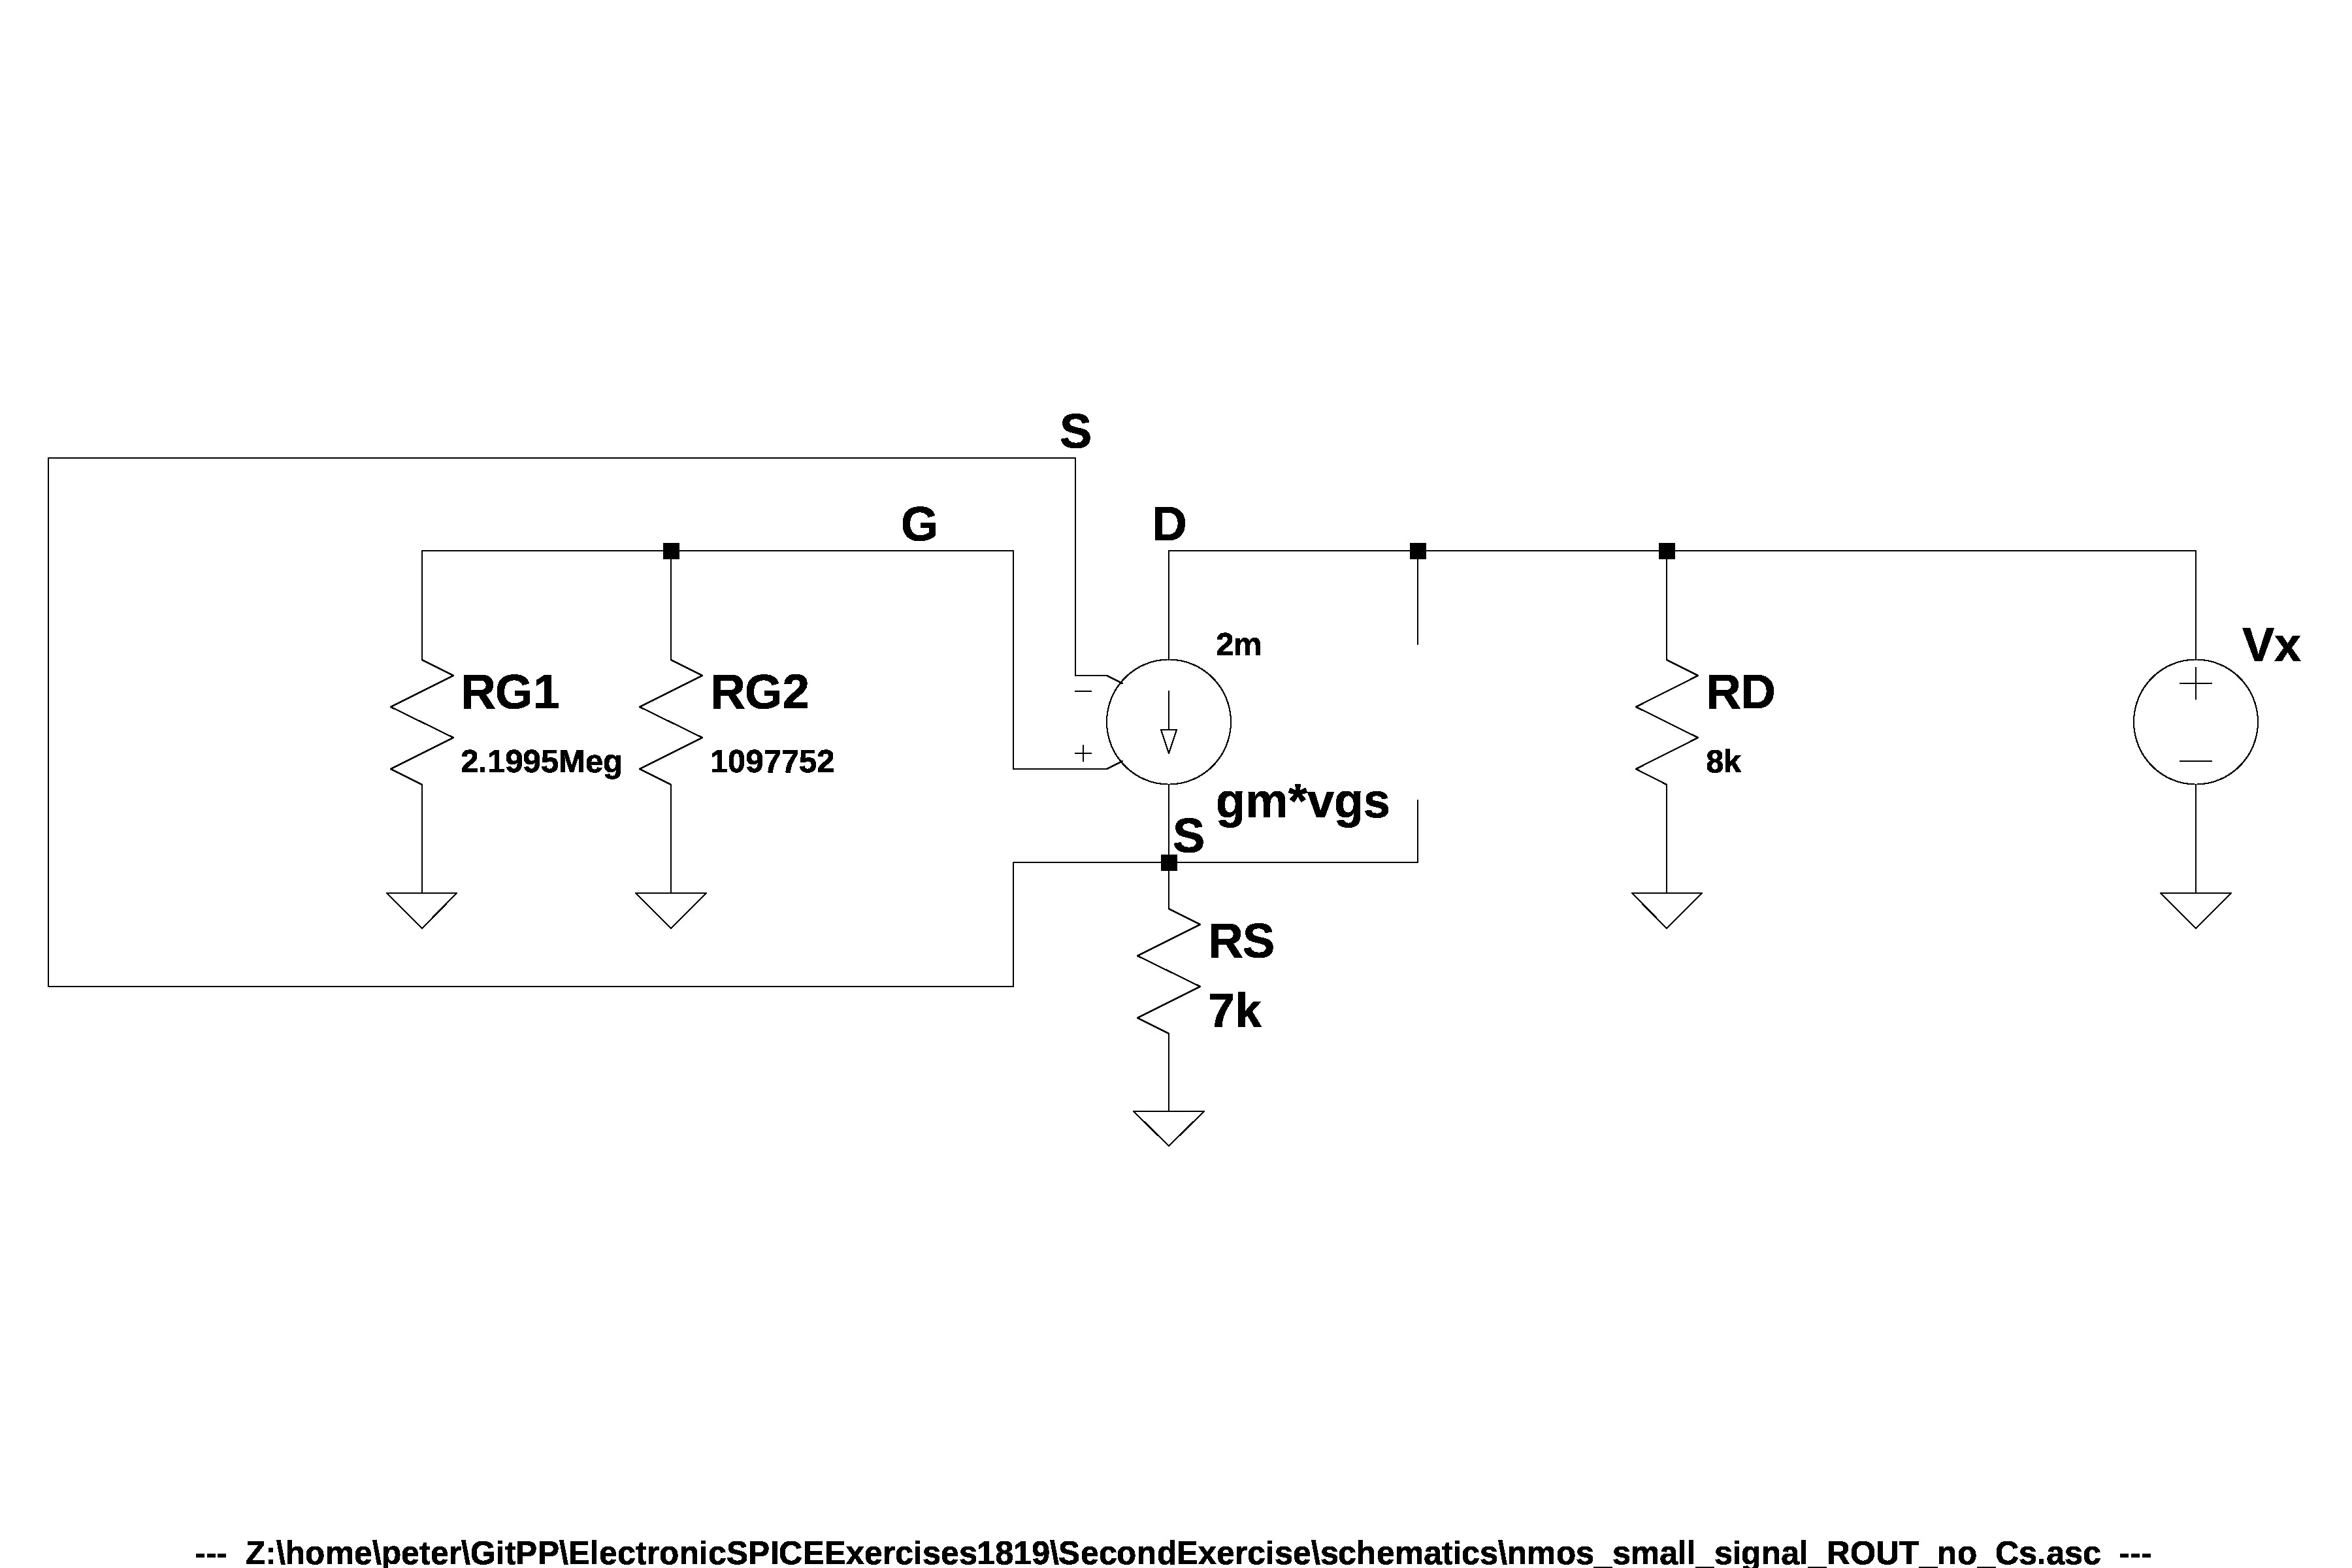
\includegraphics[width=12cm]{schematics/nmos_small_signal_ROUT_no_Cs.jpg}
  \caption{NMOS common source amplifier - Calculating $R_{OUT}$}
  \label{nmos_pi_ROUT_no_Cs}
\end{figure}

\subsubsection{Voltage Gain - without $R_{sig}$ and $R_L$}\label{AvSecNoCs}
Calculating the gain of the amplifier represented in the figure \ref{nmos_pi_gain_without_resistances_no_Cs}.

\begin{figure}[h]
  \centering
  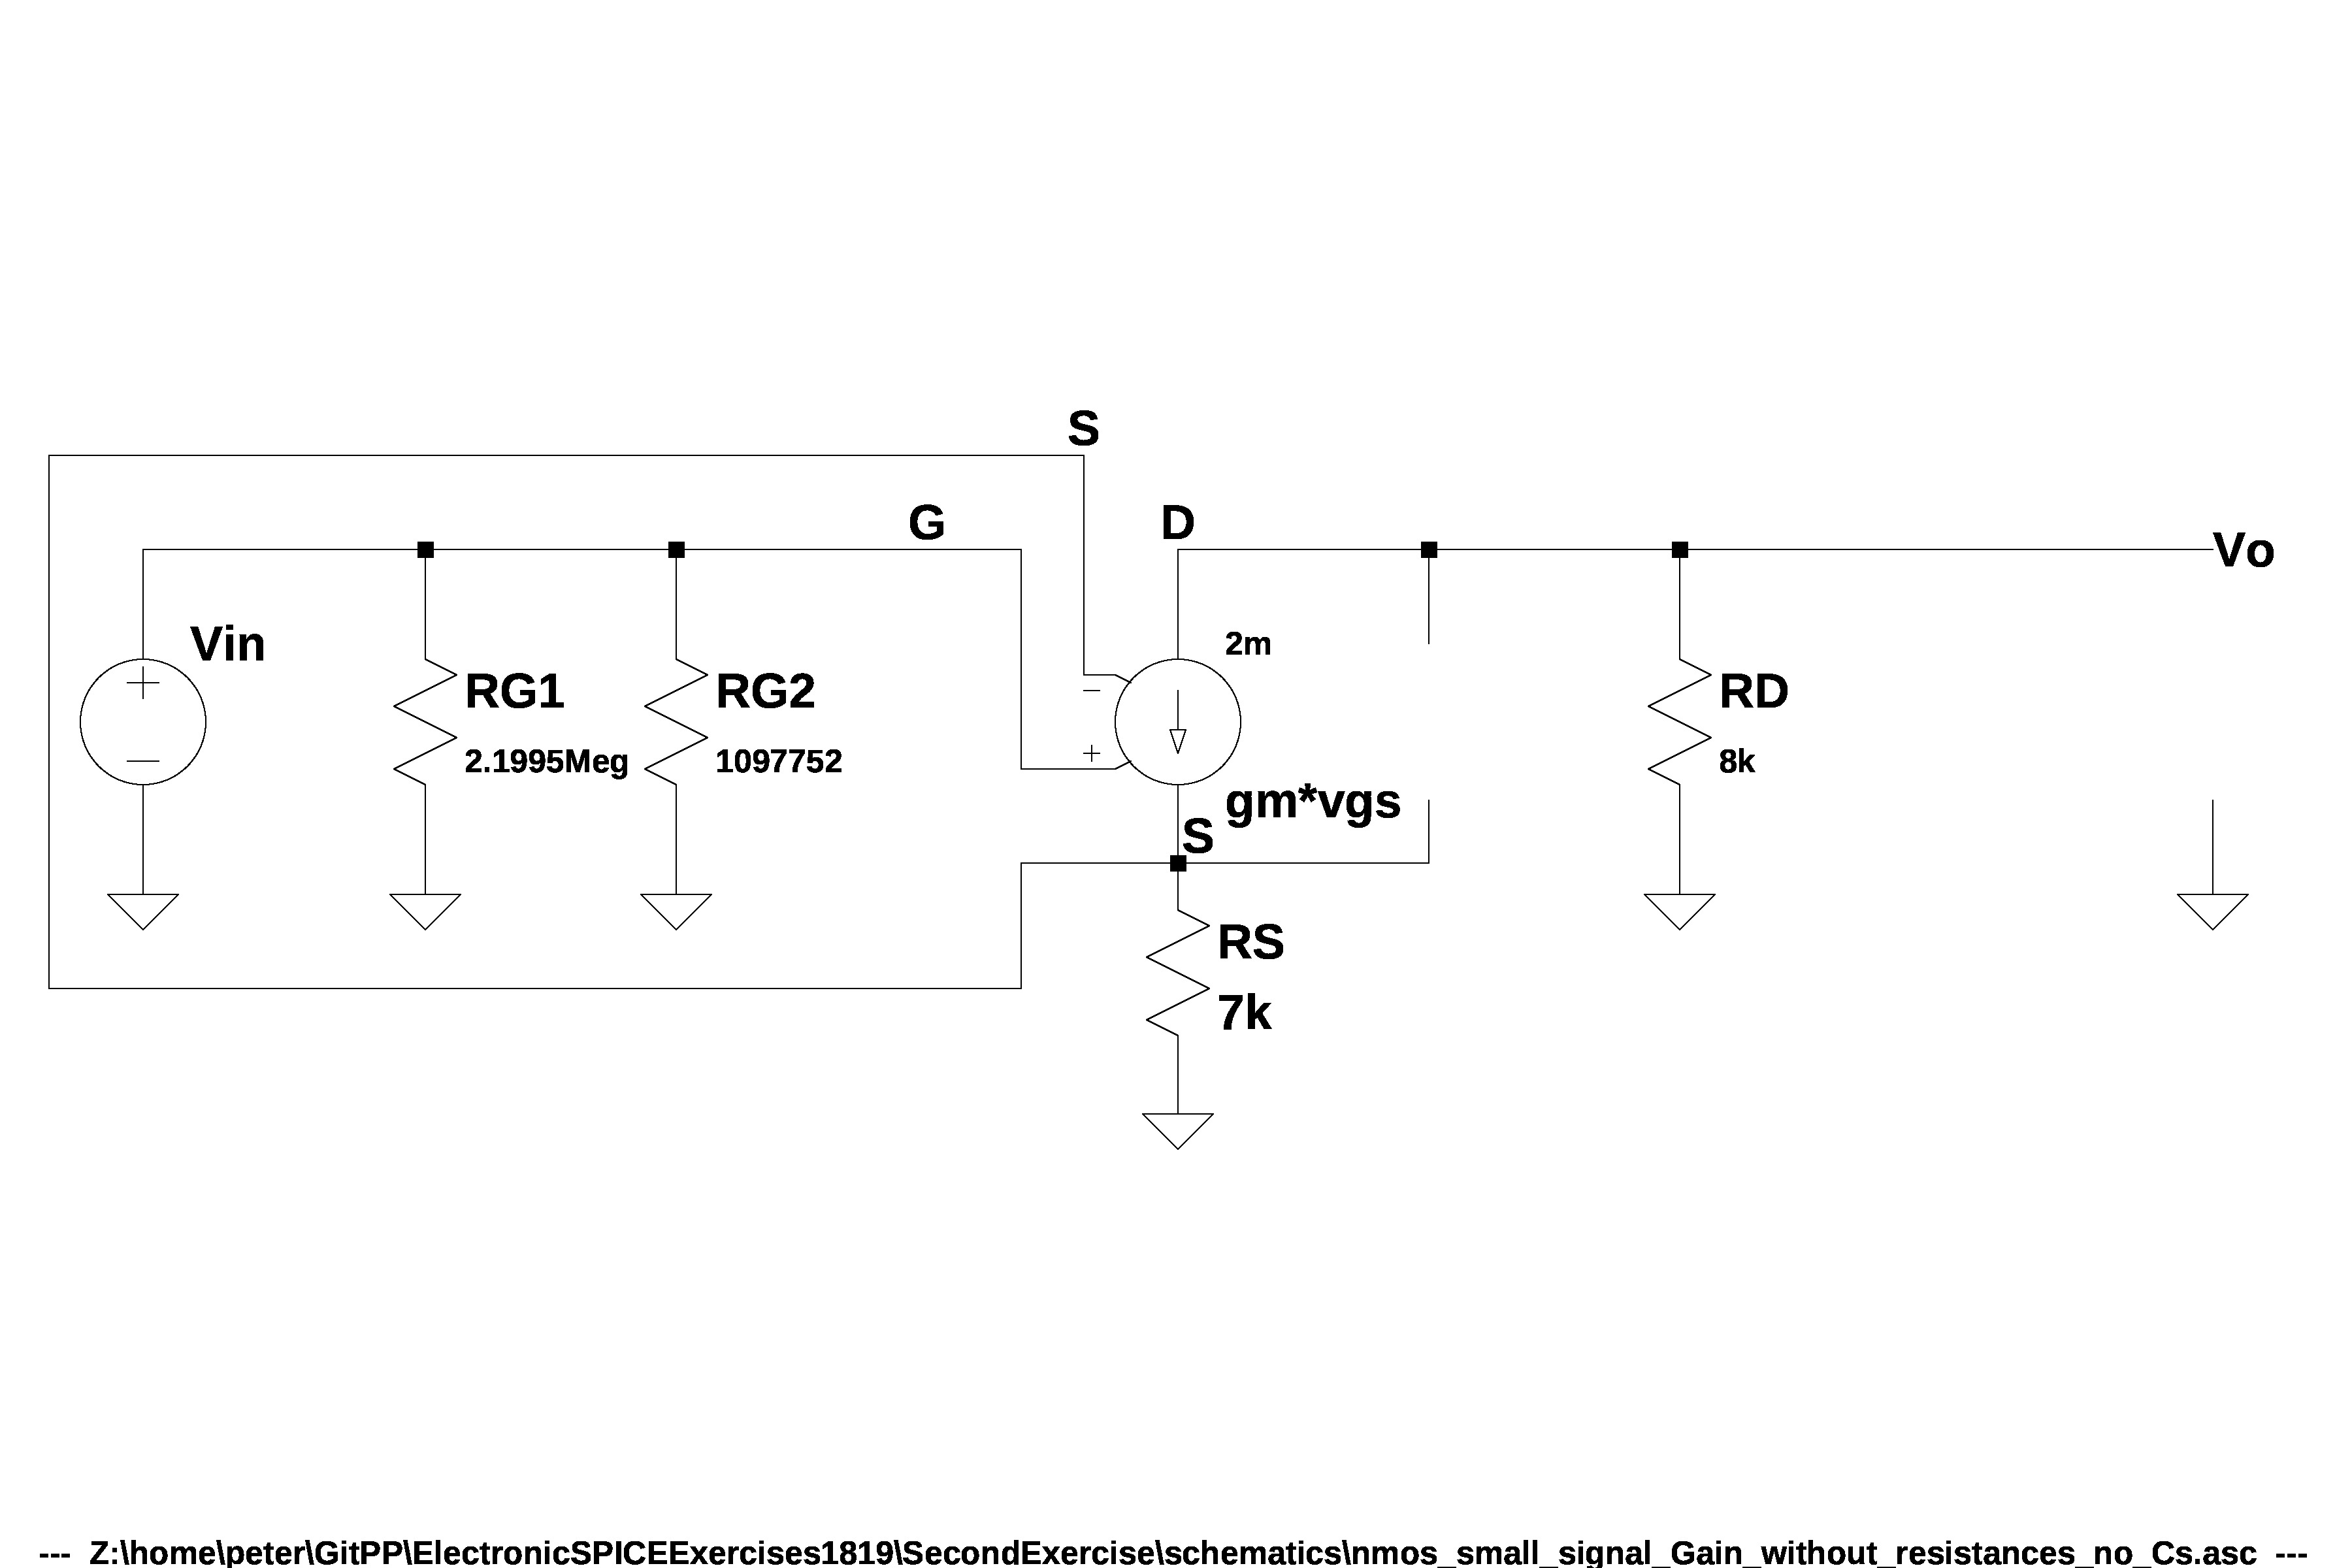
\includegraphics[width=12cm]{schematics/nmos_small_signal_without_resistances_no_Cs.jpg}
  \caption{NMOS common source amplifier - Calculating the voltage gain without $R_{sig}$ and $R_L$}
  \label{nmos_pi_gain_without_resistances_no_Cs}
\end{figure}

\begin{align}
v_{in} &= v_{g} = v_{gs}+v_s\\
&= v_{gs} + v_{gs} g_m R_S\\
&= v_{gs}(1+ g_m R_S)
\end{align}
\begin{align}
v_{o} &= - g_m v_{gs} R_D
\end{align}

\begin{align}
A_v = \frac{v_o}{v_{in}} = \frac{- g_m v_{gs} R_D}{v_{gs}(1+ g_m R_S)} = \frac{- g_m R_D}{(1+ g_m R_S)} = \frac{- 2mA/V \cdot 8k\Omega}{1+2mA/V \cdot 7k\Omega} = - 1.06667 \quad V/V \simeq - 1.1 \quad V/V \label{AvNoCs}
\end{align}

\subsubsection{Voltage Gain - with $R_{sig}$ and $R_L$}\label{GvSecNoCs}
Calculating the gain of the amplifier represented in the figure \ref{nmos_pi_gain_with_resistances_no_Cs}.

\begin{figure}[h]
  \centering
  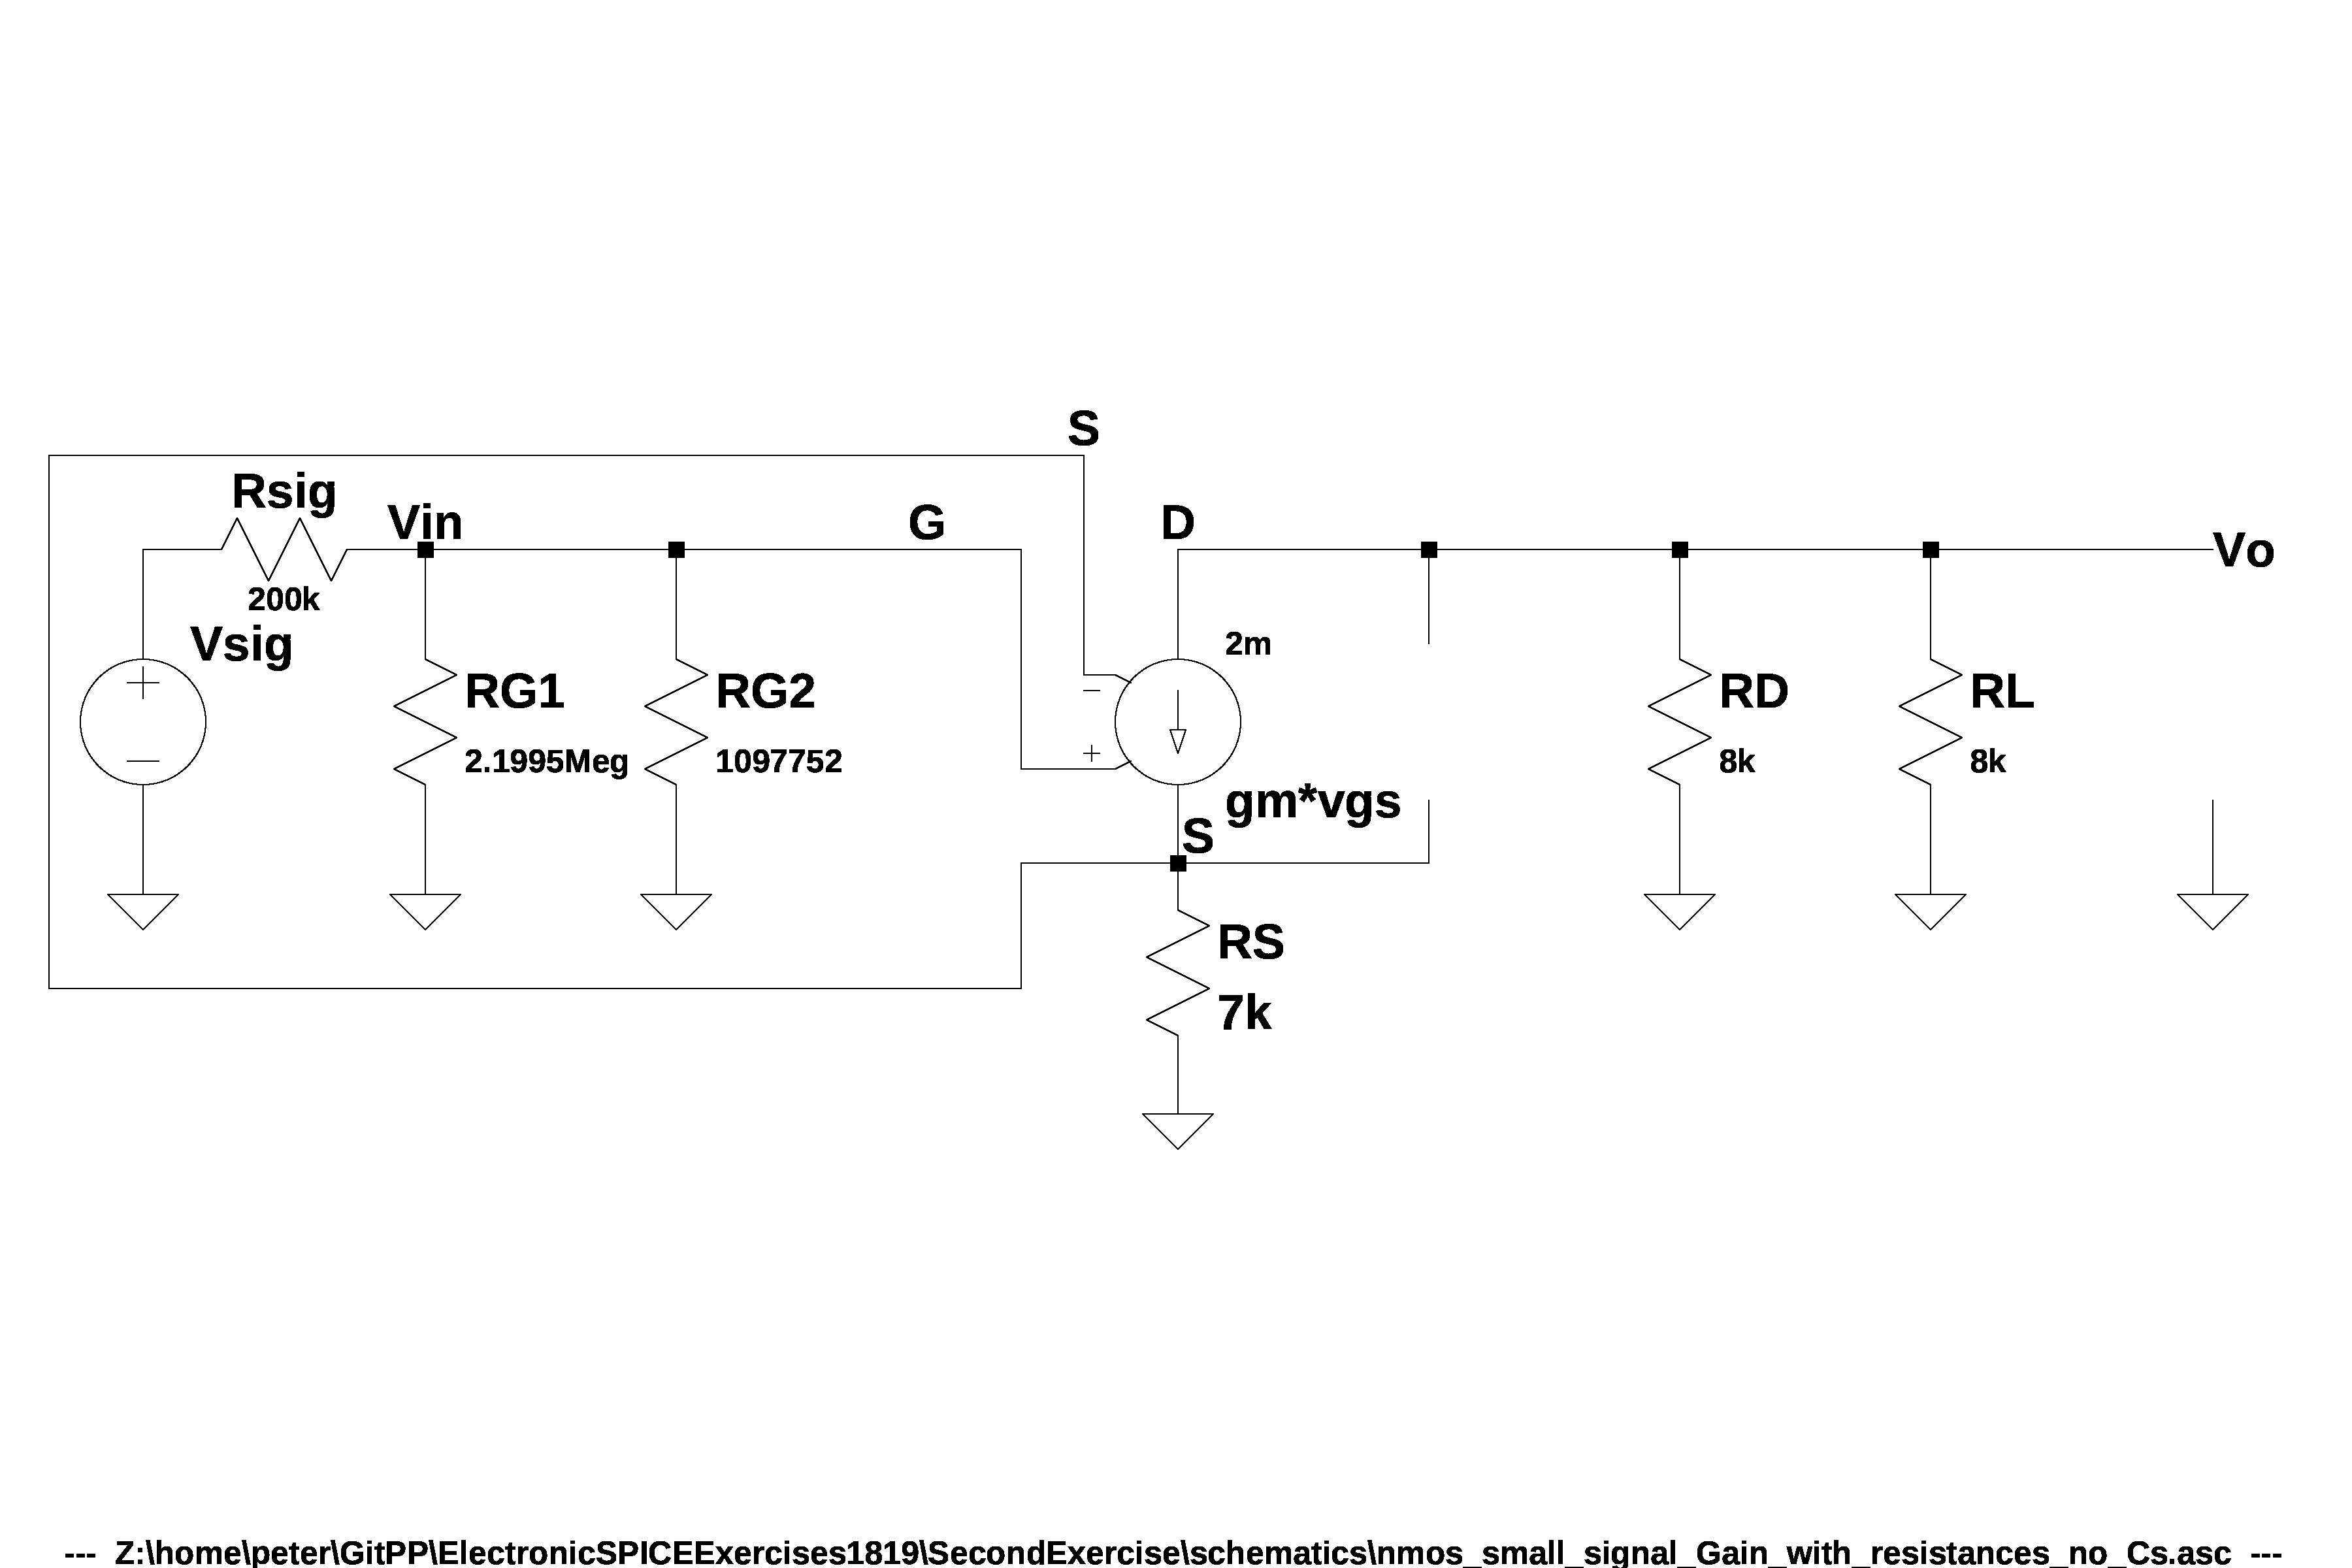
\includegraphics[width=12cm]{schematics/nmos_small_signal_with_resistances_no_Cs.jpg}
  \caption{NMOS common source amplifier - Calculating the voltage gain with $R_{sig}$ and $R_L$}
  \label{nmos_pi_gain_with_resistances_no_Cs}
\end{figure}

\begin{align}
I_{sig} &= \frac{v_{sig}}{R_{sig} + (R_{G1} \parallel R_{G2})}
\end{align}

\begin{align}
v_{in} = v_{g} &= v_{sig} - R_{sig} I_{sig}\\
&= v_{sig} - R_{sig} \frac{v_{sig}}{R_{sig} + (R_{G1} \parallel R_{G2})}\\
&= v_{sig} \left(1 - R_{sig} \frac{1}{R_{sig} + (R_{G1} \parallel R_{G2})}\right)
\end{align}

\begin{align}
v_{gs} &= v_g - v_s\\
v_{gs} &= v_{sig} \left(1 - R_{sig} \frac{1}{R_{sig} + (R_{G1} \parallel R_{G2})}\right) - g_m v_gs R_S\\
v_{gs} + g_m v_{gs} R_S &= v_{sig} \left(1 - R_{sig} \frac{1}{R_{sig} + (R_{G1} \parallel R_{G2})}\right)\\
v_{gs} (1+ g_m R_S) &= v_{sig} \left(1 - R_{sig} \frac{1}{R_{sig} + (R_{G1} \parallel R_{G2})}\right)\\
V_{gs} &= v_{sig} \left(1 - R_{sig} \frac{1}{R_{sig} + (R_{G1} \parallel R_{G2})}\right) \frac{1}{1+ g_m R_S}
\end{align}

\begin{align}
v_o &= - g_m v_{gs} (R_D \parallel R_L)\\
&= -g_m v_{sig} \left(1 - R_{sig} \frac{1}{R_{sig} + (R_{G1} \parallel R_{G2})}\right) \frac{1}{1+ g_m R_S} (R_D \parallel R_L)
\end{align}

\begin{align}
G_v = \frac{v_o}{v_{sig}} &= \frac{-g_m v_{sig} \left(1 - R_{sig} \frac{1}{R_{sig} + (R_{G1} \parallel R_{G2})}\right) \frac{1}{1+ g_m R_S} (R_D \parallel R_L)}{v_{sig}}\\
&= -g_m \left(1 - R_{sig} \frac{1}{R_{sig} + (R_{G1} \parallel R_{G2})}\right) \frac{1}{1+ g_m R_S} (R_D \parallel R_L)\\
&= \frac{-g_m}{1+ g_m R_S} \left(1 - \frac{R_{sig}}{R_{sig} + \left(\frac{R_{G1}R_{G2}}{R_{G1}+R_{G2}}\right)}\right) \left(\frac{R_{D}R_{L}}{R_{D}+R_{L}}\right)\\
&= \frac{-2mA/V}{1+ 2mA/V \cdot 7k\Omega} \left(1 - \frac{200k\Omega}{200k\Omega + \left(\frac{2.19550M\Omega \cdot 1097752\Omega}{2.19550M\Omega +1097752\Omega}\right)}\right) \left(\frac{8k\Omega \cdot 8k\Omega}{8k\Omega + 8k\Omega}\right)\\
&= -0.41886 \quad V/V \simeq -0.42 \quad V/V \label{GvNoCs}
\end{align}

\clearpage
\section{SPICE simulations}
\subsection{DC simulation - Operating Point}
Same as the section \ref{DCsim}.

\subsection{AC simulation without bypass capacitances - $Av$, $R_{IN}$ and $R_{OUT}$}
\lstinputlisting{netlist/nmos_small_signal_RIN_ROUT_no_Cs.cir}
The result confirm the analysis (result calculated in the section \ref{AvSecNoCs}, expression \ref{AvNoCs}).
\lstinputlisting{netlist/nmos_small_signal_RIN_ROUT_no_Cs.tf}

\subsection{AC simulation without bypass capacitances - $Gv$}
\lstinputlisting{netlist/nmos_small_signal_RIN_ROUT_with_Rs_Rl_no_Cs.cir}
The result confirm the analysis (result calculated in the section \ref{GvSecNoCs}, expression \ref{GvNoCs}).
\lstinputlisting{netlist/nmos_small_signal_RIN_ROUT_with_Rs_Rl_no_Cs.tf}

\end{document}
